%%%%%%%%%%%%%%%%%%%%%%%%%%%%%%%%%%%%%%%%%
% Classicthesis Typographic Thesis
% LaTeX Template
% Version 1.3 (15/2/14)
%
% This template has been downloaded from:
% http://www.LaTeXTemplates.com
%
% Original author:
% André Miede (http://www.miede.de)
%
% License:
% CC BY-NC-SA 3.0 (http://creativecommons.org/licenses/by-nc-sa/3.0/)
%
% General Tips:
% 1) Make sure to edit the classicthesis-config.file
% 2) New enumeration (A., B., C., etc in small caps): \begin{aenumerate} \end{aenumerate}
% 3) For margin notes: \marginpar or \graffito{}
% 4) Do not use bold fonts in this style, it is designed around them
% 5) Use tables as in the examples
% 6) See classicthesis-preamble.sty for useful commands
%
%%%%%%%%%%%%%%%%%%%%%%%%%%%%%%%%%%%%%%%%%

%----------------------------------------------------------------------------------------
%	PACKAGES AND OTHER DOCUMENT CONFIGURATIONS
%----------------------------------------------------------------------------------------

\documentclass[
		twoside,openright,titlepage,numbers=noenddot,headinclude,%1headlines,
                footinclude=true,cleardoublepage=empty,
                BCOR=5mm,paper=a4,fontsize=11pt, % Binding correction, paper type and font size
                ngerman,american, % Languages
                ]{scrreprt} 
                
% Includes the file which contains all the document configurations and packages - make sure to edit this file
%%%%%%%%%%%%%%%%%%%%%%%%%%%%%%%%%%%%%%%%%
% Thesis Configuration File
%
% The main lines to change in this file are in the DOCUMENT VARIABLES
% section, the rest of the file is for advanced configuration.
%
%%%%%%%%%%%%%%%%%%%%%%%%%%%%%%%%%%%%%%%%%

%----------------------------------------------------------------------------------------
%	DOCUMENT VARIABLES
%	Fill in the lines below to enter your information into the thesis template
%	Each of the commands can be cited anywhere in the thesis
%----------------------------------------------------------------------------------------

% Remove drafting to get rid of the '[ Date - classicthesis version 4.0 ]' text at the bottom of every page
\PassOptionsToPackage{eulerchapternumbers,listings,drafting, pdfspacing, subfig,beramono,parts}{classicthesis}
% Available options: drafting parts nochapters linedheaders eulerchapternumbers beramono eulermath pdfspacing minionprospacing tocaligned dottedtoc manychapters listings floatperchapter subfig
% Adding 'dottedtoc' will make page numbers in the table of contents flushed right with dots leading to them

\newcommand{\myTitle}{A new approach to Economic Geography}
\newcommand{\mySubtitle}{An Homage to The Elements of Typographic Style\xspace}
\newcommand{\myDegree}{Docteur en Physique Th\'eorique\xspace}
\newcommand{\myName}{R\'emi Louf\xspace}
\newcommand{\myProf}{Marc Barthelemy\xspace}
\newcommand{\myOtherProf}{Put name here\xspace}
\newcommand{\mySupervisor}{Put name here\xspace}
\newcommand{\myFaculty}{Put data here\xspace}
\newcommand{\myDepartment}{Put data here\xspace}
\newcommand{\myUni}{Université Pierre et Marie Curie\xspace}
\newcommand{\myLocation}{Darmstadt\xspace}
\newcommand{\myTime}{June 2015\xspace}
\newcommand{\myVersion}{version 1.0\xspace}

%----------------------------------------------------------------------------------------
%	USEFUL COMMANDS
%----------------------------------------------------------------------------------------

\newcommand{\ie}{i.\,e.}
\newcommand{\Ie}{I.\,e.}
\newcommand{\eg}{e.\,g.}
\newcommand{\Eg}{E.\,g.} 

\newcounter{dummy} % Necessary for correct hyperlinks (to index, bib, etc.)
\providecommand{\mLyX}{L\kern-.1667em\lower.25em\hbox{Y}\kern-.125emX\@}

%----------------------------------------------------------------------------------------
%	PACKAGES
%----------------------------------------------------------------------------------------

\usepackage{lipsum} % Used for inserting dummy 'Lorem ipsum' text into the template

%------------------------------------------------
 
\PassOptionsToPackage{latin9}{inputenc} % latin9 (ISO-8859-9) = latin1+"Euro sign"
\usepackage{inputenc}
 
 %------------------------------------------------

%\PassOptionsToPackage{ngerman,american}{babel}  % Change this to your language(s)
% Spanish languages need extra options in order to work with this template
%\PassOptionsToPackage{spanish,es-lcroman}{babel}
\usepackage{babel}

%------------------------------------------------			

\PassOptionsToPackage{square,numbers}{natbib}
 \usepackage{natbib}
 
 %------------------------------------------------

\PassOptionsToPackage{fleqn}{amsmath} % Math environments and more by the AMS 
 \usepackage{amsmath}
 
 %------------------------------------------------

\PassOptionsToPackage{T1}{fontenc} % T2A for cyrillics
\usepackage{fontenc}

%------------------------------------------------

\usepackage{xspace} % To get the spacing after macros right

%------------------------------------------------

\usepackage{mparhack} % To get marginpar right

%------------------------------------------------

\usepackage{fixltx2e} % Fixes some LaTeX stuff 

%------------------------------------------------

\PassOptionsToPackage{smaller}{acronym} % Include printonlyused in the first bracket to only show acronyms used in the text
\usepackage{acronym} % nice macros for handling all acronyms in the thesis

%------------------------------------------------

%\renewcommand*{\acsfont}[1]{\textssc{#1}} % For MinionPro
\renewcommand{\bflabel}[1]{{#1}\hfill} % Fix the list of acronyms

%------------------------------------------------

\PassOptionsToPackage{pdftex}{graphicx}
\usepackage{graphicx} 

%----------------------------------------------------------------------------------------
%	FLOATS: TABLES, FIGURES AND CAPTIONS SETUP
%----------------------------------------------------------------------------------------

\usepackage{tabularx} % Better tables
\setlength{\extrarowheight}{3pt} % Increase table row height
\newcommand{\tableheadline}[1]{\multicolumn{1}{c}{\spacedlowsmallcaps{#1}}}
\newcommand{\myfloatalign}{\centering} % To be used with each float for alignment
\usepackage{caption}
\captionsetup{format=hang,font=small}
\usepackage{subfig}  

%----------------------------------------------------------------------------------------
%	CODE LISTINGS SETUP
%----------------------------------------------------------------------------------------

\usepackage{listings} 
%\lstset{emph={trueIndex,root},emphstyle=\color{BlueViolet}}%\underbar} % for special keywords
\lstset{language=[LaTeX]Tex, % Specify the language for listings here
keywordstyle=\color{RoyalBlue}, % Add \bfseries for bold
basicstyle=\small\ttfamily, % Makes listings a smaller font size and a different font
%identifierstyle=\color{NavyBlue}, % Color of text inside brackets
commentstyle=\color{Green}\ttfamily, % Color of comments
stringstyle=\rmfamily, % Font type to use for strings
numbers=left, % Change left to none to remove line numbers
numberstyle=\scriptsize, % Font size of the line numbers
stepnumber=5, % Increment of line numbers
numbersep=8pt, % Distance of line numbers from code listing
showstringspaces=false, % Sets whether spaces in strings should appear underlined
breaklines=true, % Force the code to stay in the confines of the listing box
%frameround=ftff, % Uncomment for rounded frame
frame=single, % Frame border - none/leftline/topline/bottomline/lines/single/shadowbox/L
belowcaptionskip=.75\baselineskip % Space after the "Listing #: Desciption" text and the listing box
}

%----------------------------------------------------------------------------------------
%	HYPERREFERENCES
%----------------------------------------------------------------------------------------

\PassOptionsToPackage{pdftex,hyperfootnotes=false,pdfpagelabels}{hyperref}
\usepackage{hyperref}  % backref linktocpage pagebackref
\pdfcompresslevel=9
\pdfadjustspacing=1

\hypersetup{
% Uncomment the line below to remove all links (to references, figures, tables, etc)
%draft, 
colorlinks=true, linktocpage=true, pdfstartpage=3, pdfstartview=FitV,
% Uncomment the line below if you want to have black links (e.g. for printing black and white)
%colorlinks=false, linktocpage=false, pdfborder={0 0 0}, pdfstartpage=3, pdfstartview=FitV, 
breaklinks=true, pdfpagemode=UseNone, pageanchor=true, pdfpagemode=UseOutlines,
plainpages=false, bookmarksnumbered, bookmarksopen=true, bookmarksopenlevel=1,
hypertexnames=true, pdfhighlight=/O, urlcolor=webbrown, linkcolor=RoyalBlue, citecolor=webgreen,
%------------------------------------------------
% PDF file meta-information
pdftitle={\myTitle},
pdfauthor={\textcopyright\ \myName, \myUni, \myFaculty},
pdfsubject={},
pdfkeywords={},
pdfcreator={pdfLaTeX},
pdfproducer={LaTeX with hyperref and classicthesis}
%------------------------------------------------
}   

%----------------------------------------------------------------------------------------
%	BACKREFERENCES
%----------------------------------------------------------------------------------------

\usepackage{ifthen} % Allows the user of the \ifthenelse command
\newboolean{enable-backrefs} % Variable to enable backrefs in the bibliography
\setboolean{enable-backrefs}{false} % Variable value: true or false

\newcommand{\backrefnotcitedstring}{\relax} % (Not cited.)
\newcommand{\backrefcitedsinglestring}[1]{(Cited on page~#1.)}
\newcommand{\backrefcitedmultistring}[1]{(Cited on pages~#1.)}
\ifthenelse{\boolean{enable-backrefs}} % If backrefs were enabled
{
\PassOptionsToPackage{hyperpageref}{backref}
\usepackage{backref} % to be loaded after hyperref package 
\renewcommand{\backreftwosep}{ and~} % separate 2 pages
\renewcommand{\backreflastsep}{, and~} % separate last of longer list
\renewcommand*{\backref}[1]{}  % disable standard
\renewcommand*{\backrefalt}[4]{% detailed backref
\ifcase #1 
\backrefnotcitedstring
\or
\backrefcitedsinglestring{#2}
\else
\backrefcitedmultistring{#2}
\fi}
}{\relax} 

%----------------------------------------------------------------------------------------
%	AUTOREFERENCES SETUP
%	Redefines how references in text are prefaced for different 
%	languages (e.g. "Section 1.2" or "section 1.2")
%----------------------------------------------------------------------------------------

\makeatletter
\@ifpackageloaded{babel}
{
\addto\extrasamerican{
\renewcommand*{\figureautorefname}{Figure}
\renewcommand*{\tableautorefname}{Table}
\renewcommand*{\partautorefname}{Part}
\renewcommand*{\chapterautorefname}{Chapter}
\renewcommand*{\sectionautorefname}{Section}
\renewcommand*{\subsectionautorefname}{Section}
\renewcommand*{\subsubsectionautorefname}{Section}
}
\addto\extrasngerman{
\renewcommand*{\paragraphautorefname}{Absatz}
\renewcommand*{\subparagraphautorefname}{Unterabsatz}
\renewcommand*{\footnoteautorefname}{Fu\"snote}
\renewcommand*{\FancyVerbLineautorefname}{Zeile}
\renewcommand*{\theoremautorefname}{Theorem}
\renewcommand*{\appendixautorefname}{Anhang}
\renewcommand*{\equationautorefname}{Gleichung}
\renewcommand*{\itemautorefname}{Punkt}
}
\providecommand{\subfigureautorefname}{\figureautorefname} % Fix to getting autorefs for subfigures right
}{\relax}
\makeatother

%----------------------------------------------------------------------------------------

\usepackage{classicthesis} 
%----------------------------------------------------------------------------------------
%	CHANGING TEXT AREA 
%----------------------------------------------------------------------------------------

%\linespread{1.05} % a bit more for Palatino
%\areaset[current]{312pt}{761pt} % 686 (factor 2.2) + 33 head + 42 head \the\footskip
%\setlength{\marginparwidth}{7em}%
%\setlength{\marginparsep}{2em}%

%----------------------------------------------------------------------------------------
%	USING DIFFERENT FONTS
%----------------------------------------------------------------------------------------

%\usepackage[oldstylenums]{kpfonts} % oldstyle notextcomp
%\usepackage[osf]{libertine}
\usepackage{hfoldsty} % Computer Modern with osf
%\usepackage[light,condensed,math]{iwona}
%\renewcommand{\sfdefault}{iwona}
%\usepackage{lmodern} % <-- no osf support :-(
%\usepackage{MnSymbol}
\usepackage{MinionPro}
%\usepackage[urw-garamond]{mathdesign} <-- no osf support :-(


\begin{document}

\frenchspacing % Reduces space after periods to make text more compact

\raggedbottom % Makes all pages the height of the text on that page

\selectlanguage{american} % Select your default language - e.g. american or ngerman

%\renewcommand*{\bibname}{new name} % Uncomment to change the name of the bibliography
%\setbibpreamble{} % Uncomment to include a preamble to the bibliography - some text before the reference list starts

\pagenumbering{roman} % Roman page numbering prior to the start of the thesis content (i, ii, iii, etc)

\pagestyle{plain} % Suppress headers for the pre-content pages

%----------------------------------------------------------------------------------------
%	PRE-CONTENT THESIS PAGES
%----------------------------------------------------------------------------------------

% Title Page

\begin{titlepage}

\begin{addmargin}[-1cm]{-3cm}
\begin{center}
\large

\hfill
\vfill

\begingroup
\color{Maroon}\spacedallcaps{\myTitle} \\ \bigskip % Thesis title
\endgroup

\spacedlowsmallcaps{\myName} % Your name

\vfill


\includegraphics[width=6cm]{gfx/TFZsuperellipse_bw} \\ \medskip % Picture

\mySubtitle \\ \medskip % Thesis subtitle
%\myDegree \\
%\myDepartment \\
%\myFaculty \\
%\myUni \\ \bigskip

\myTime\ -- \myVersion % Time and version

\vfill

\end{center}
\end{addmargin}

\end{titlepage} % Main title page
% Back of the title page

\thispagestyle{empty}

\hfill

\vfill

\noindent\myName: \textit{\myTitle,} \mySubtitle, %\myDegree, 
\textcopyright\ \myTime

% You may wish to do something with the back of the title page, such as including your supervisors, location or time frame of the work. Below is an example of doing so although you may want to tweak it to your liking.

%\bigskip

%\noindent\spacedlowsmallcaps{Supervisors}: \\
%\myProf \\
%\myOtherProf \\ 
%\mySupervisor

%\medskip \\

%\noindent\spacedlowsmallcaps{Location}: \\
%\myLocation

%\medskip \\

%\noindent\spacedlowsmallcaps{Time Frame}: \\
%\myTime
 % Back of the title page
\cleardoublepage% Dedication

\thispagestyle{empty}
\refstepcounter{dummy}

\pdfbookmark[1]{Dedication}{Dedication} % Bookmark name visible in a PDF viewer

\vspace*{3cm}

\begin{center}
    I had the idea that the world's so full of pain \\
	it must sometimes make a kind of singing. \\ \medskip
    --- Robert Hass,\, \emph{Faint Music}    
\end{center}

\bigskip

\begin{center}
    \`A mes parents. \\ \smallskip
    Qui ont toujours plac\'e l'\'education avant tout.
\end{center}

\bigskip

\begin{center}
   To Hannah. \\ \smallskip
   (line intentionally left blank)
\end{center}
 % Dedication page
\cleardoublepage% Abstract

\pdfbookmark[1]{Abstract}{Abstract} % Bookmark name visible in a PDF viewer

\begingroup
\let\clearpage\relax
\let\cleardoublepage\relax
\let\cleardoublepage\relax

\chapter*{Abstract} % Abstract name

Short summary of the contents\dots

\endgroup			

\vfill % Abstract page
\cleardoublepage% Publications - a page listing research articles written using content in the thesis

\pdfbookmark[1]{Publications}{Publications} % Bookmark name visible in a PDF viewer

\chapter*{Publications} % Publications page text

Some ideas and figures have appeared previously in the following publications:

\bigskip

\noindent Put your publications from the thesis here. The packages \texttt{multibib} or \texttt{bibtopic} etc. can be used to handle multiple different bibliographies in your document. % Publications from the thesis page
\cleardoublepage% Acknowledgements

\pdfbookmark[1]{Acknowledgements}{Acknowledgements} % Bookmark name visible in a PDF viewer

\begin{flushright}{\slshape    
    [T]outes mes conduites \'etaient surd\'etermin\'ees\\
    par la d\'esolation intime du deuil solitaire:\\
    le travail fou \'etait aussi une mani\`ere \\
    de combler un immense vide et de sortir du d\'esespoir\\
    en prenant int\'r\^et aux autres.} \\ \medskip
    --- \defcitealias{Bourdieu:2001}{Pierre Bourdieu}\citetalias{Bourdieu:2001} \citep{Bourdieu:2001}
\end{flushright}

\begingroup

\let\clearpage\relax
\let\cleardoublepage\relax
\let\cleardoublepage\relax

\chapter*{Acknowledgements} % Acknowledgements section text

List of people to thank

\begin{itemize}
	\item Thomas
	\item Hannah
	\item Benoit
        \item Hadrien
        \item Clement
	\item Riccardo and Giulia
	\item secretaries
	\item Ed
	\item Arianna
	\item Marie and Olivia
	\item Elisa
	\item Bruno
	\item Rosa-L\'y
        \item The Linacre College Boat Club, for accepting me back in a boat,
            despite my poor fitness after $3$ years of intense PhD. For letting
            me row at Oxford's Summer VIII's and replace horrible thoughts about
            my dissertation by equally horrible though about erging.
\end{itemize}

\noindent Many thanks to the Open Source community, without which I would not
have been able to do even a half of this thesis. The developpers behind linux,
for providing such a stable and efficient system. The developpers of Python and
of the many python libraries. All the work I have done has been made possible by
the selfless work of many before me.


\endgroup
 % Acknowledgements page

\pagestyle{scrheadings} % Show chapter titles as headings
\cleardoublepage% Table of Contents - List of Tables/Figures/Listings and Acronyms

\refstepcounter{dummy}

\pdfbookmark[1]{\contentsname}{tableofcontents} % Bookmark name visible in a PDF viewer

\setcounter{tocdepth}{2} % Depth of sections to include in the table of contents - currently up to subsections

\setcounter{secnumdepth}{3} % Depth of sections to number in the text itself - currently up to subsubsections

\manualmark
\markboth{\spacedlowsmallcaps{\contentsname}}{\spacedlowsmallcaps{\contentsname}}
\tableofcontents 
\automark[section]{chapter}
\renewcommand{\chaptermark}[1]{\markboth{\spacedlowsmallcaps{#1}}{\spacedlowsmallcaps{#1}}}
\renewcommand{\sectionmark}[1]{\markright{\thesection\enspace\spacedlowsmallcaps{#1}}}

\clearpage

\begingroup 
\let\clearpage\relax
\let\cleardoublepage\relax
\let\cleardoublepage\relax

    
       
%----------------------------------------------------------------------------------------
%	Acronyms
%----------------------------------------------------------------------------------------

\refstepcounter{dummy}
%\addcontentsline{toc}{chapter}{Acronyms} % Uncomment if you would like the acronyms to appear in the table of contents
\pdfbookmark[1]{Acronyms}{acronyms} % Bookmark name visible in a PDF viewer

\markboth{\spacedlowsmallcaps{Acronyms}}{\spacedlowsmallcaps{Acronyms}}

\chapter*{Acronyms}

\begin{acronym}[UML]
\acro{MSA}{Metropolitan Statistical Areas}
\acro{CBSA}{Combined Statistical Area}
\acro{UA}{Urban Areas}
\end{acronym}  
                   
\endgroup
 % Contents, list of figures/tables/listings and acronyms

\cleardoublepage

\pagenumbering{arabic} % Arabic page numbering for thesis content (1, 2, 3, etc)
%\setcounter{page}{90} % Uncomment to manually start the page counter at an arbitrary value (for example if you wish to count the pre-content pages in the page count)

\cleardoublepage % Avoids problems with pdfbookmark

%----------------------------------------------------------------------------------------
%	THESIS CONTENT - CHAPTERS
%----------------------------------------------------------------------------------------

\ctparttext{The study of urban systems is changing at a fast pace, due to the
use of new sources of data. Or is it really? In this part, I will briefly
outline the history of the quantitative tradition in the study of urban systems,
and argue that we may be witnessing a second quantitative revolution. I will
briefly expose the methodoly, giving concrete examples of why this methodology
should be followed. I end the part with a collection of puzzles about urban
systems that I attempt to solve in the rest of the manuscript.} % Text on the Part 1 page describing  the content in Part 1

\part{Introduction} % First part of the thesis

% Introduction

\pdfbookmark[1]{Introduction}{Introduction}


\chapter{Quantitative revolution(s) in urban science}
\label{chap:quantitative_revolutions}

\begin{flushright}{\slshape    
And the first one now\\
Will later be last\\
For the times they are a-changin'} \\ \medskip
--- Bob Dylan 
\end{flushright}

\section{The first quantitative revolution}
\label{sec:the_first_quantitative_revolution}


\section{A second quantitative revolution?}
\label{sec:a_second_quantitative_revolution_}


    \subsection{New methods}
    \label{sub:new_methods}


    \subsection{New data}
    \label{sub:new_data}
    
    \subsection{A technological convergence}
    \label{sub:a_technological_convergence} 
 % Chapter 1
% Introduction

\pdfbookmark[1]{Introduction}{Introduction}

\chapter{Methodology}
\label{chap:methodology}

\begin{flushright}{\slshape    
If it disagrees with experiment, it's wrong.\\ 
In that simple statement is the key to science.} \\ \medskip
--- Richard Feynman 
\end{flushright}

\section{The importance of being naive}
\label{sec:the_importance_of_being_naive}

\section{In defense of reductionism}
\label{sec:in_defense_of_reductionism}

In fact, we do not need to have a full theoretical description of the human mind
to say something about the actions of hundreds of thousands, a million of them.
In the same way we do not need string theory in order to explain the
functioning of living organisms.

\section{Quantitative stands for 'data'}
\label{sec:quantitative_stands_for_data_}

\section{Against data}
\label{sec:against_data}

In `Againt Method', the philosopher of science Paul Feyerabend argued against
the idea that Science proceeds through the application of a single, monolithic
method; what people usually call `The Scientific Method'. The reference is not
innocent, and I will argue here that, although empirical analysis constitutes
the alpha and the omega of our enquiry for knowledge, data are not enough.  

% Introduction

\pdfbookmark[1]{Introduction}{Introduction}

\chapter{About this thesis}
\label{chap:methodology}

\begin{flushright}{\slshape    
Creativity is more than just being different.\\
Anybody can plan weird; that's easy.
} \\ \medskip
--- Charles Mingus 
\end{flushright}


\section{Some puzzles}

\section{Outline}

\section{Style of the thesis}

I will be using the pronoun 'we' for most of the manuscript, to reflect the fact
that the work presented here was often done in the context of collaboration with others. A
notable exception is the part concerning the systems of cities, where all the
research is mine.


\cleardoublepage % Empty page before the start of the next part

%------------------------------------------------

\ctparttext{The model of the monocentric city, an idealisation of urban systems
where all activities are organised around a single center, still pervades the
literature on urban systems. The contribution of this part is twofolds. We first
demonstrate empirically that large cities are indeed organised around several
centers, and propose an alternative measure to the traditional `distance to the
center' measure. We then propose a model to explain the emergence of several
centers as cities expand, and test the predictions of this model against
available data.} % Text on the Part 2 page describing the content in Part 2

\part{The (end of the) monocentric city} % Second part of the thesis

% !TEX root = ../thesis-example.tex
%
\chapter{The (end of the) monocentric city}
\label{sec:related}

\cleanchapterquote{A picture is worth a thousand words. An interface is worth a thousand pictures.}{Ben Shneiderman}{(Professor for Computer Science)}

\section{Introduction}
\label{sec:introduction}

\section{How congestion shapes cities}
\label{sec:how_congestion_shapes_cities}

Empirical evidence suggest that most urban systems experience a
transition from a monocentric to a polycentric organisation as they
grow and expand. We propose here a stochastic, out-of-equilibrium model of the
city which explains the appearance of subcenters as an effect of
traffic congestion. We show that congestion triggers the unstability
of the monocentric regime, and that the number of subcenters and the
total commuting distance within a city scale sublinearly with its
population, predictions which are in agreement with data gathered for
around 9000 US cities between 1994 and 2010.\\


As cities grow, they evolve from a monocentric organisation where all
the activities are concentrated in the same geographical area
--usually the central business district-- to a more distributed,
polycentric organisation
~\cite{Kemper:1974,Odland:1978,Mills:1972,Griffith_PG:1981,Dokmeci:1994,McMillen:2003,Pereira:2013,Roth:2011}. Traditional
approaches in spatial economics have attempted to describe the
phenomenon within the framework of equilibrium models of the city~\cite{Fujita:1982,Fujita:book1999}. These models are traditionally
based on the concept of agglomeration economies --to explain why
economical activities tend to group-- and the spatial distribution of
wages and rents across the urban space. However, these approaches fail
at giving a satisfactory quantitative
account~\cite{Bouchaud:2008,Batty:2008} of the polycentric transition
of cities. First, they describe a city as being in an equilibrium
characterised by static spatial distributions of households and business
firms. However, the equilibrium assumption is unsupported as cities
are out-of-equilibrium systems and their
dynamics is of particular interest for practical
applications~\cite{Batty:2008}. Second, these models integrate so many
interactions and variables that it is difficult to understand the
hierarchy of processes governing the evolution of cities, which ones are fundamental and which ones a irrelevant. Yet, traffic congestion is not
explicitly taken into account in the existing models, despite being
mentioned in the economics literature as a possible reason for the
polycentric transition~\cite{McMillen:2003}. Lastly, the models do
not make any quantitative prediction and are therefore unsupported by
data.\\ 
We present in this Letter a stochastic, out-of-equilibrium model of the
city which relies on the assumption that the polycentric structure of
large cities might find its origin in congestion, irrespective of the
particular local economic details. We are able to reproduce many
stylized facts, and --most importantly-- to derive a general relation
between the number of activity centers of a city and its
population. Finally, we verify this relation against the employment
data from around 9000 cities in the US between 1994 and 2010.

%\section{The model}

Following recent interdisciplinary efforts to construct a quantitative
description of cities and their
evolution~\cite{Makse:1995,Zanette:1997,Marsili:1998a,Marsili:1998b,Batty:book2005,Bettencourt:2007,Batty:2008},
we deliberately omit certain details and focus instead on basic
processes. We thereby aim at building a minimal model which captures
the complexity of the system and is able to account for --qualitative as well as quantitive-- stylized
facts. The model we propose is by essence dynamical and describes the
evolution of cities' organisation as their population increases. We
focus on car congestion --mainly due to journey-to-work commutes --
and its effect on the job location choice for individuals.

According to Fujita and Ogawa's classical model~\cite{Fujita:1982} in
spatial economics, an individual living at location $i$ will choose to
work at the location $j$ which maximises the net income after
deduction of the rent and commuting costs~\cite{Fujita:1982}
%
\begin{equation}
Z_0=W(j)-C_R(i)-C_T(i,j)
\end{equation} 
%
where $W(j)$ is the average wage paid by business firms located at $j$
(and thus varies from a location to another), $C_R(i)$ is the land
rent at $i$, and $C_T(i,j)$ is the commuting cost between $i$ and
$j$. The wage and the land rent result from the interplay between
household and companies locations, agglomeration effects being taken
into account. The commuting cost, on the other hand, does not usually take congestion 
into account and is taken proportional to the euclidean distance
$C_T(i,j) = t\, d_{ij}$ (where $t$ is the transportation cost per unit
of distance) in most studies.

The time scales involved in the evolution of cities are usually such
that the employment turnover rate is larger than the relocation
rate of households. On a short time scale, we can thus focus on the
process of job-seeking alone, leaving aside the problem of the choice of
residence. In other words, we assume the coupling between both processes to be negligible: we assume that each
inhabitant newly added to the city has a random residence location and
we concentrate on understanding how such an inhabitant chooses its job
among a pool of $N_c$ potential activity centers (which we suppose are also
randomly distributed among the city). The active subcenters are then defined as the subset of potential centers which have a non zero incoming number of
individuals. As a result of these assumptions, a worker living at $i$
will choose to work at the center $j$ such that the quantity
%
\begin{equation}
Z_{ij} = W(j) - C_T(i,j)
\end{equation}
%
is maximum. \\
We now discuss the form of the two terms $W(j)$ and
$C_T$. The problem of determining the (spatial) variations of the
average wage $W(j)$ at location $j$ is very reminiscent of some
problems encountered in fundamental physics. Indeed, the wage depends
on many different factors, ranging from the type of company, the
education level of the inhabitant, the level of aglomeration, etc.,
and in this respect is not too different from quantities that can be
measured in a large atom made of a large number of interacting
particles. In this situation, physicists found out that although it is possible
to write down the corresponding equations, not only is it
impossible to solve them, but also not really useful. In fact they
found out~\cite{Dyson:1962} that a statistical description of these
systems, relying on random matrices could lead to predictions which agree with experimental results. We wish to import in spatial economics
this idea of replacing a complex quantity such as wages --which depends on
so many factors and interactions-- by a random one. We therefore decide to
account for the interaction between activity centers and people by
taking the wage as proportional to a random variable $\eta_j \in \left[ 0,1\right]$
such that $W(j) = s\, \eta_j$ where $s$ defines the maximum attainable
average wage in the considered city.

As for the transportation cost $C_T(i,j)$, we choose it to be
proportional to the commuting time between $i$ and $j$. In a typical
situation where passenger transportation is dominated by personal
vehicles, this commuting time not only depends on the distance between
the two places, but also on the traffic between $i$ and $j$, the vehicle capacity of
the underlying network and its resilience to congestion. The Bureau of
Public Road formula~\cite{Branston:1976} proposes a simple form taking
all these ingredients into account. In our framework, it leads to the following expression for the 
commuting costs
%
\begin{equation}
C_T(i,j) =  t\, d_{ij} \left[ 1 + \left( \frac{T_{ij}}{c} \right)^{\mu} \right]
\end{equation}
%
where $T_{ij}$ the trafic per unit of time between $i$ and $j$ and $c$
is the typical capacity of a road (taken constant here). The quantity
$\mu$ is a parameter quantifying the resilience of the transportation
network to congestion. We further simplify the problem by assuming
than the traffic $T_{ij}$ is only a function of the subcenter $j$ and
therefore write $T_{ij}=T(j)$ the total traffic incoming in subcenter
$j$ (see Supplementary Material~\cite{SM} for a short discussion).

In summary, our model is defined as follows. At each time step, we add
a new individual $i$ located at random in the city, who will
choose to work in the activity area $j$ (among $N_c$ possibilities
located at random) such that the following quantity
%
\begin{equation}
Z_{ij} = \eta_j - \frac{d_{ij}}{\ell} \left[ 1 + \left( \frac{T(j)}{c} \right)^{\mu} \right]
\label{eq:cost_function}
\end{equation}
%
is maximum (we omitted irrelevant multiplicative factors). The quantity $\ell = s/t$ is interpreted as the maximum effective
commuting distance that people can financially withstand. 


Depending on the relative importance of wages, distance and congestion, the
model predicts the existence of three different regimes: the monocentric
regime (top Fig.~\ref{fig:model_results}), the distance-driven polycentric (middle Fig.~\ref{fig:model_results}) regime
and the attractivity-driven polycentric (bottom Fig.~\ref{fig:model_results}) regime. 


\begin{figure}
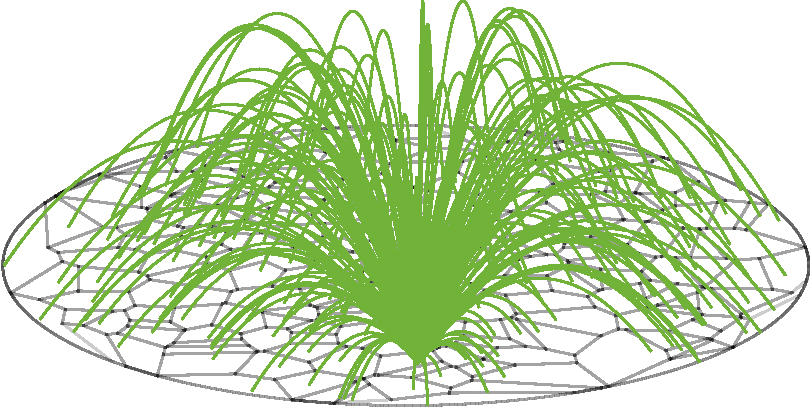
\includegraphics[width=0.4\textwidth]{gfx/chapter-monocentric/1.pdf}
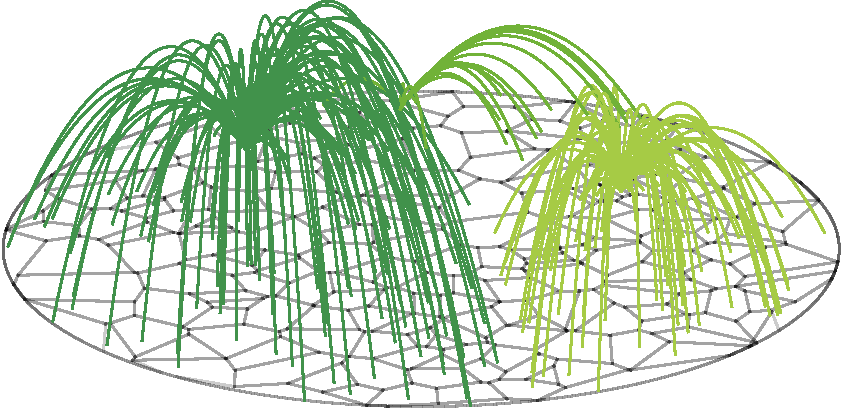
\includegraphics[width=0.4\textwidth]{gfx/chapter-monocentric/2.pdf}
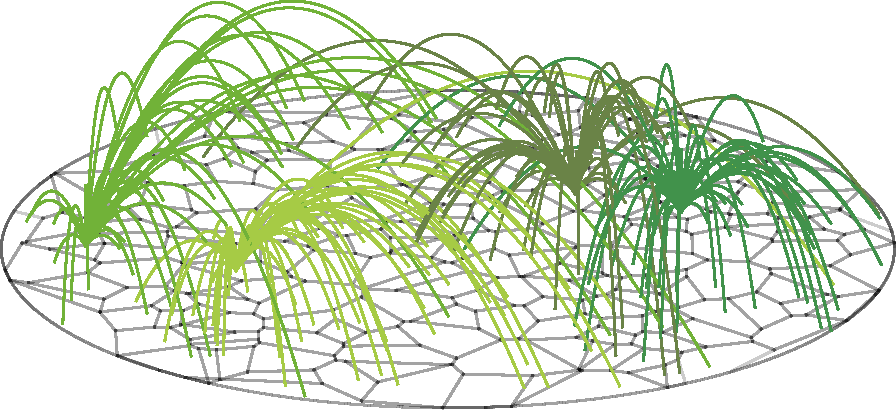
\includegraphics[width=0.4\textwidth]{gfx/chapter-monocentric/3.pdf}
\caption{The monocentric (top), distance-driven polycentric (middle)
  and attractivity-driven polycentric (bottom) regimes as produced by
  our model. Each link represents a commuting journey to an activity center. \label{fig:model_results}}
\end{figure}


From now on, we will assume that $\ell$ is large enough so that a
monocentric state exists for small values of the population. In this
regime, the value of $\eta$ prevails and the monocentric state evolves
to an attractivity-driven polycentric structure as the population
increases (if $\ell$ is too small, the monocentric regime does not
exist-see the Supplementary material~\cite{SM} for more details on
these points).  Starting from a small city with a monocentric
organisation, the traffic is negligible and $Z_{ij}\approx \eta_j$
which implies that all individual are going to choose the most
attractive center (with the largest value of $\eta_j$, say
$\eta_1$). When the number $P$ of households increases, the traffic
will also increase and some initially less attractive centers (with
smaller values of $\eta$) might become more attractive, leading to the
appearance of new subcenters characterized by a non-zero number of
commuters. More precisely, a new subcenter $j$ will appear when for an
individual $i$, we have $Z_{ij}>Z_{i1}$. The traffic so far is
$T(1)=P$ and $T(j)=0$ which leads to the equation
\begin{equation}
\eta_j-\frac{d_{ij}}{\ell}>\eta_1-\frac{d_{i1}}{\ell}\left[1+\left(\frac{P}{c}\right)^\mu\right]
\end{equation}
We assume that there are no spatial
correlations in the subcenter distribution, so that we can make the
approximation $d_{ij}\sim d_{i1}\sim L$. The new subcenter will thus
be such that $\eta_1-\eta_j$ is minimum implying that it will have the
second largest value denoted by $\eta_j=\eta_2$. For a uniform distribution
(details of the calculation can be found in the Supplementary
Material~\cite{SM}, section 2), on average
$\overline{\eta_1-\eta_2}\simeq 1/N_c$ leading to a critical value for
the population
%
\begin{equation}
P^*= c \left( \frac{\ell}{L N_c} \right)^{1/\mu}
\end{equation}
%
Whatever the system considered, there will therefore \emph{always} be
a critical value of the population above which the city becomes
polycentric (which can be smaller than one, in which case there is no
monocentric regime at all, see the Supplementary Material~\cite{SM}). The monocentric regime is therefore fundamentally
unstable with regards to population increase, which is in agreement with the fact that no major city in
the world exhibits a monocentric structure. We note that the smaller
the value of $\mu$ (or larger the value of the capacity $c$), the
larger the critical population value $P^*$ which means that cities
with a good road system capable of absorbing large traffic display a
monocentric structure for a longer period of time.


Having established that cities will eventually adopt a polycentric
structure, we can wonder how the number of subcenters varies with the
population. We compute the value of the population at which 
the $k^{th}$ center appears. We still assume that we are in the attractivity-driven regime and that, so far, $k-1$
centers have emerged with $\eta_{1} \geq \eta_{2} \geq ... \geq
\eta_{k-1}$~\cite{SM}, with a number of commuters $T(1), T(2), ...,
T(k-1)$, respectively. The next worker $i$ will choose the center $k$ if
\begin{equation}
Z_{ik} > \max_{j \in \left[1,k-1\right]} Z_{ij}
\end{equation}
which reads
\begin{equation}
\eta_k - \frac{d_{ik}}{\ell} > \max_{j \in \left[1,k-1\right]} \left\{
\eta_j - \frac{d_{ij}}{\ell} \left[ 1 + \left(
  \frac{T(j)}{c}\right)^\mu\right] \right\}
\end{equation}
The distribution of traffic $T(j)$ is narrow~\cite{SM}, which means that all the centers have roughly the same number of
commuters $T(j) \sim P/(k-1)$. As above we also assume that the
distance between the workers' households and the activity centers is
typically $d_{ij} \sim d_{ik} \sim L$. The previous expression now
reads
\begin{equation}
\frac{L}{\ell} \left( \frac{P}{(k-1)\,c} \right)^{\mu} > \max_{j \in
  \left[1,k-1\right]} \left( \eta_j \right) - \eta_k
\end{equation}
Following our definitions, $\max_{j \in \left[1,k-1\right]} \left(
\eta_j \right) = \eta_1$. According to order statistics, if the
$\eta_j$ are uniformly distributed, we have on average
$\overline{\eta_1 - \eta_k} = (k-1)/(N_c+1)$. It follows from these
assumptions that (1) the $k^{th}$ center to appear is the $k^{th}$ most attractive one (2) the average value of the population $\overline{P}_k$ at
which the $k^{th}$ center appears is given by:
%
\begin{equation}
\overline{P}_k = P^* \left( k-1 \right)^{\frac{\mu+1}{\mu}}
\label{eq:prediction}
\end{equation}
%
Conversely, the number $k$ of subcenters scales sublinearly with population as
\begin{equation}
k \sim \left( \frac{\overline{P}}{P^*} \right)^{\frac{\mu}{\mu + 1}}
\end{equation}
It is interesting to note that this result is robust: the dependence
is sublinear, \emph{whatever the distribution} of the random variable
$\eta$ (see the Supplementary Material~\cite{SM} for a discussion on this
point). We can therefore conclude that, probably very generally and
under mild assumptions, the number of activity subcenters in urban
areas scales sublinearly with their population where the prefactor and
the exponent depend on the properties of the transportation network of
the city under consideration. 

A previous study~\cite{Samaniego:2008} showed that the daily total
miles driven daily in a city --- the `total commuting
distance'---scales with the population as $L_{tot} \sim P^\gamma$
where $\gamma \in \left] 0.5, 1\right[$, which the authors interpreted
as cities having neither a neither totally centralized nor totally
decentralized structure. We can discuss this result within the
framework of our model in the following way. If the system was in the
pure attractivity-driven regime, we would have $L_{tot} \sim P$. But, if we
assume that we are in an intermediate regime where
Eq.~\ref{eq:prediction} holds, and where the system exhibits spatial
coherence~\cite{SM}, we can write the total length of commuting
journeys as
%
\begin{equation}
L_{tot} \sim P \frac{L}{\sqrt{k}}
\end{equation} 
%
Inverting the result from Eq.~\ref{eq:prediction} we therefore get
%
\begin{equation}
L_{tot} \sim P^{1-\frac{\beta}{2}}
\label{eq:beta}
\end{equation}
%
where $\beta = \frac{\mu}{\mu+1} \in \left[0 , 1\right]$. Our model is
thus consistent with the fact that the total traveled miles scales with
population with a non-trivial exponent comprised in $[0.5,1]$.\\


\begin{figure*}
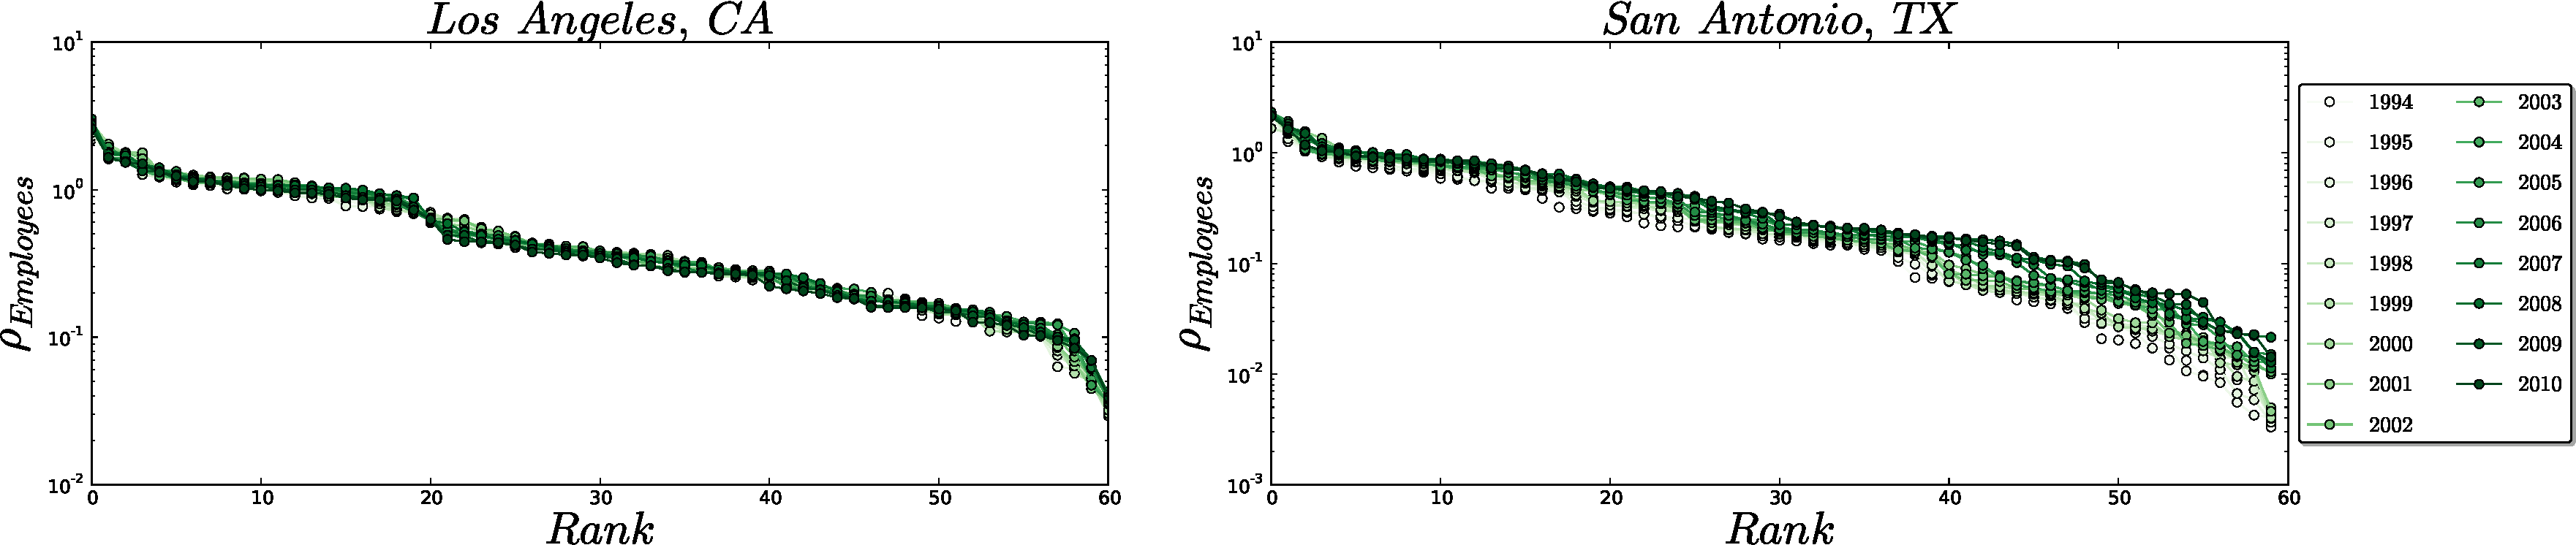
\includegraphics[width=\textwidth]{gfx/chapter-monocentric/4.pdf}
\caption{Rank-plot for the employment density (in employees per
  $km^2$) in Los Angeles, CA (left) and San Antonio, TX (right)
  between 1994 and 2010. See the Supplementary Material~\cite{SM} for more details. \label{fig:rank_plots}}
\end{figure*}

    \subsection{Empirical verification}
    \label{sub:empirical_verification}
    
People from the Census Bureau use the 2000 Census tract-to-tract commuting data
in order to get the employment density~\cite{Marlay:2010}. Use these data in
order to assess the employment density in 2000 MSAs. Use population data at the
same level in order to assess population density in 2000 MSAs.
Plot at several levels of the threshold and show the many different centers.
Propose a method to compute the number of centers (exponential, Loubar...).\\
        \subsubsection{Counting the number of centers}
        \label{ssub:counting_the_number_of_centers}
        
        
We now test the prediction given by Eq. (\ref{eq:prediction}). For
that purpose, we collected data for the number of employees per Zip
Codes in the United States for 16 years, between 1994 and
2010~\cite{ZBPdata}, as well as the population of all cities in the US
between 1994 and 2010~\cite{CensusData}. We estimate the number of
subcenters by constructing the rank-plot of the employment density
$\rho$ (number of employees per $km^2$) for each Zip Code of a given
urban area~\cite{Griffith:1981,Dokmeci:1994}. These plots display a decay as fast as an exponential
(Fig.~\ref{fig:rank_plots}) which implies that there exists a natural
scale for the rank, that we interpret here as the typical number of
activity centers. It also implies that any reasonable method should
give an estimate of the number of subcenters of the same order of
magnitude (which would not be the case for slowly decaying function
such as power laws for example). We first note that for some cities
--typically large ones with stable populations
(Fig.~\ref{fig:rank_plots}, left)-- the employment spatial statistics
remained stable over the period of study. For other cities, we observe
large variation of the number of subcenters
(Fig.~\ref{fig:rank_plots}, right). We then plot (Fig.~\ref{fig:data})
the population $P$ of cities (with population $P>100$) versus the
estimated number of subcenters $k$ (the dispersion in the scatterplot
probably results from the fact that different cities have different
resilience levels to congestion). On average, we observe a power law
dependance with exponent $\delta=1.56 \pm 0.15$ (the result is robust
with regards to the estimate of $k$, see the Supplementary
Material~\cite{SM} for more details). Inverting this relation gives us
the number of subcenters as a function of the population
%
\begin{equation}
k \sim P^{\beta}
\end{equation}
%
with $\beta \sim 0.64$. This result is strikingly in agreement with
the prediction given by our model: the number of subcenters in a city
scales sublinearly with its population.\\

\begin{figure}
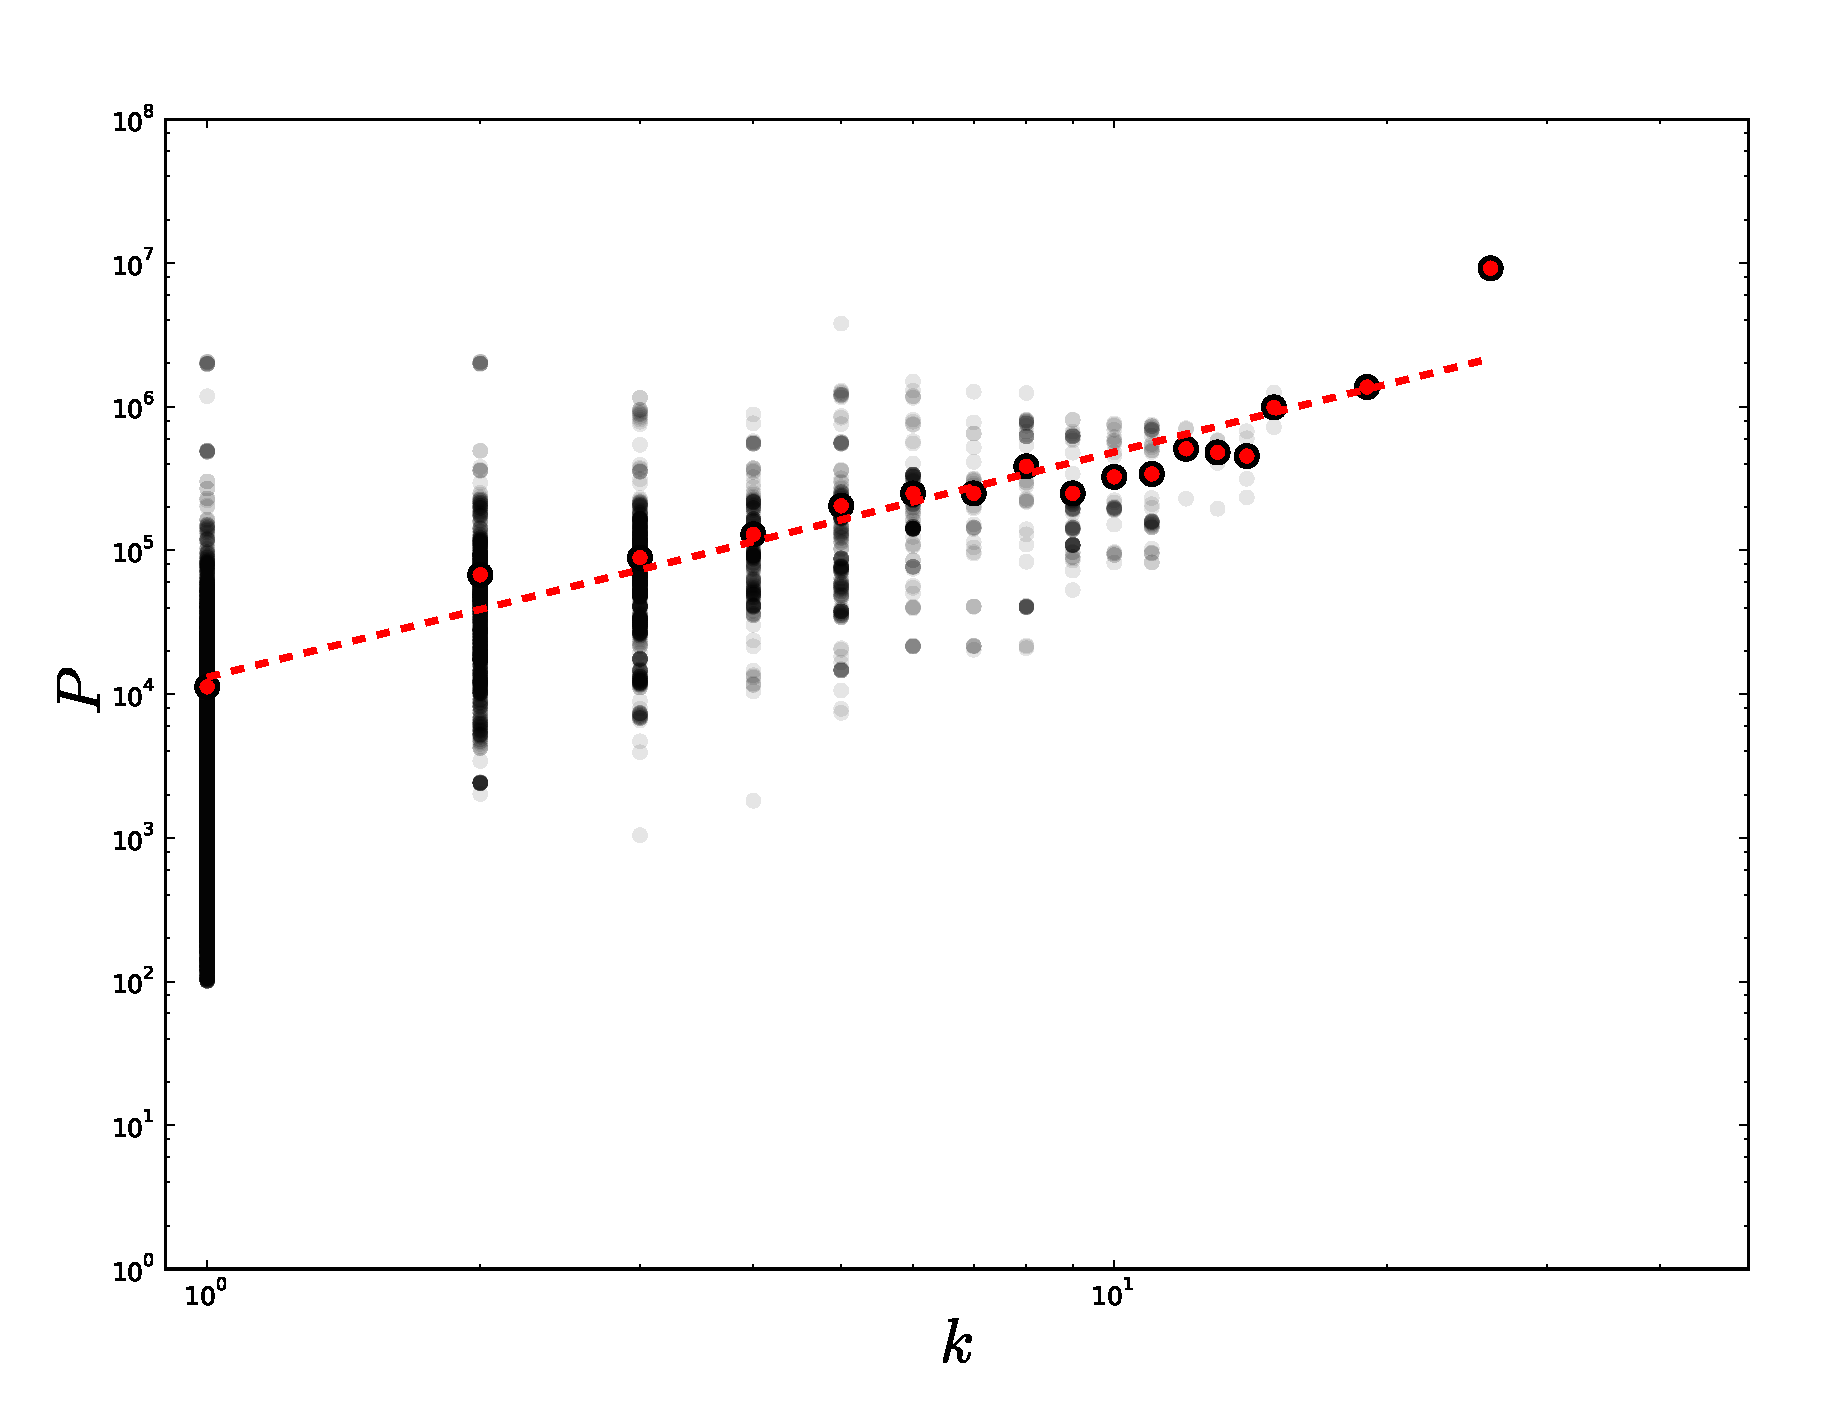
\includegraphics[width=0.5\textwidth]{gfx/chapter-monocentric/5.pdf}
\caption{Scatter plot of the estimated number of subcenters versus the
  population for about 9000 cities with population over 100 people in
  the US. The red dots represent the average population for a given
  number of subcenters. We fit this average with a power-law
  dependence (represented by a red dashed line) giving an exponent
  $\delta=1.56\pm 0.15$ ($r^2=0.87$). See the Supplementary Material~\cite{SM} for more details on the computation of $k$ and the robustness of the results. \label{fig:data}}
\end{figure}

Using the measured value of $\beta$ and Eq. (\ref{eq:beta}) we can estimate the exponent of
the scaling of $L_{tot}$ with the population and find $L_{tot} \sim
P^{\,0.68}$ which agrees very well with the value $0.66$ measured
in~\cite{Samaniego:2008} directly on the data of the daily total miles
driven in more than $400$ cities in the US.\\

While agglomeration economies seem to be the basic process explaining
the existence of cities and their spectacular resilience, this study
brings evidence that congestion is the driving force that tears them
apart. The non trivial spatial patterns observed in large cities can
thus be understood as a result of the interplay between these
competing processes. We believe that the present model represents an
important step towards a quantitative, predictive science of
cities. More generally, this microscopic approach is an interesting
example of an out-of-equilibrium model: it is governed by local
optimization with saturation effects, leads to different regimes, and
is characterized by non-trivial dynamical exponents. In this respect,
we believe that this discrete approach might be of use in the study of
pattern formation in biology --which have been so far explored from a
global optimisation perspective~\cite{Ashton:2005} or using
coarse-grained reaction-diffusion approaches with density dependent
diffusion coefficients~\cite{Cates:2012}-- to compute quantities that
are out of reach within the current methods.
\section{Proviso}
\label{sec:proviso}


 % Chapter 2

%------------------------------------------------

\ctparttext{Scaling of indicators with the population size of the city has been
recently re-discovered and explored by the different communities. In this part,
the contribution are threefold. First, a review of the exisiting literature,
pre- and post-2007 on scalings and their interpretation. Then, a model to
explain the scaling of several indicators related to mobility in cities. We then
discuss some results, Zahavi's constant and Newman and Kenworthy's famous curve.
Finally, we show that scalings pose the question of how we should define cities
as systems.} % Text on the Part 2 page describing the content in Part 2

\part{Scaling in cities} % Second part of the thesis

% !TEX root = ../thesis-example.tex
%
\chapter{The (end of the) monocentric city}
\label{sec:related}

\cleanchapterquote{A picture is worth a thousand words. An interface is worth a thousand pictures.}{Ben Shneiderman}{(Professor for Computer Science)}

\section{Introduction}
\label{sec:introduction}

\section{How congestion shapes cities}
\label{sec:how_congestion_shapes_cities}

Empirical evidence suggest that most urban systems experience a
transition from a monocentric to a polycentric organisation as they
grow and expand. We propose here a stochastic, out-of-equilibrium model of the
city which explains the appearance of subcenters as an effect of
traffic congestion. We show that congestion triggers the unstability
of the monocentric regime, and that the number of subcenters and the
total commuting distance within a city scale sublinearly with its
population, predictions which are in agreement with data gathered for
around 9000 US cities between 1994 and 2010.\\


As cities grow, they evolve from a monocentric organisation where all
the activities are concentrated in the same geographical area
--usually the central business district-- to a more distributed,
polycentric organisation
~\cite{Kemper:1974,Odland:1978,Mills:1972,Griffith_PG:1981,Dokmeci:1994,McMillen:2003,Pereira:2013,Roth:2011}. Traditional
approaches in spatial economics have attempted to describe the
phenomenon within the framework of equilibrium models of the city~\cite{Fujita:1982,Fujita:book1999}. These models are traditionally
based on the concept of agglomeration economies --to explain why
economical activities tend to group-- and the spatial distribution of
wages and rents across the urban space. However, these approaches fail
at giving a satisfactory quantitative
account~\cite{Bouchaud:2008,Batty:2008} of the polycentric transition
of cities. First, they describe a city as being in an equilibrium
characterised by static spatial distributions of households and business
firms. However, the equilibrium assumption is unsupported as cities
are out-of-equilibrium systems and their
dynamics is of particular interest for practical
applications~\cite{Batty:2008}. Second, these models integrate so many
interactions and variables that it is difficult to understand the
hierarchy of processes governing the evolution of cities, which ones are fundamental and which ones a irrelevant. Yet, traffic congestion is not
explicitly taken into account in the existing models, despite being
mentioned in the economics literature as a possible reason for the
polycentric transition~\cite{McMillen:2003}. Lastly, the models do
not make any quantitative prediction and are therefore unsupported by
data.\\ 
We present in this Letter a stochastic, out-of-equilibrium model of the
city which relies on the assumption that the polycentric structure of
large cities might find its origin in congestion, irrespective of the
particular local economic details. We are able to reproduce many
stylized facts, and --most importantly-- to derive a general relation
between the number of activity centers of a city and its
population. Finally, we verify this relation against the employment
data from around 9000 cities in the US between 1994 and 2010.

%\section{The model}

Following recent interdisciplinary efforts to construct a quantitative
description of cities and their
evolution~\cite{Makse:1995,Zanette:1997,Marsili:1998a,Marsili:1998b,Batty:book2005,Bettencourt:2007,Batty:2008},
we deliberately omit certain details and focus instead on basic
processes. We thereby aim at building a minimal model which captures
the complexity of the system and is able to account for --qualitative as well as quantitive-- stylized
facts. The model we propose is by essence dynamical and describes the
evolution of cities' organisation as their population increases. We
focus on car congestion --mainly due to journey-to-work commutes --
and its effect on the job location choice for individuals.

According to Fujita and Ogawa's classical model~\cite{Fujita:1982} in
spatial economics, an individual living at location $i$ will choose to
work at the location $j$ which maximises the net income after
deduction of the rent and commuting costs~\cite{Fujita:1982}
%
\begin{equation}
Z_0=W(j)-C_R(i)-C_T(i,j)
\end{equation} 
%
where $W(j)$ is the average wage paid by business firms located at $j$
(and thus varies from a location to another), $C_R(i)$ is the land
rent at $i$, and $C_T(i,j)$ is the commuting cost between $i$ and
$j$. The wage and the land rent result from the interplay between
household and companies locations, agglomeration effects being taken
into account. The commuting cost, on the other hand, does not usually take congestion 
into account and is taken proportional to the euclidean distance
$C_T(i,j) = t\, d_{ij}$ (where $t$ is the transportation cost per unit
of distance) in most studies.

The time scales involved in the evolution of cities are usually such
that the employment turnover rate is larger than the relocation
rate of households. On a short time scale, we can thus focus on the
process of job-seeking alone, leaving aside the problem of the choice of
residence. In other words, we assume the coupling between both processes to be negligible: we assume that each
inhabitant newly added to the city has a random residence location and
we concentrate on understanding how such an inhabitant chooses its job
among a pool of $N_c$ potential activity centers (which we suppose are also
randomly distributed among the city). The active subcenters are then defined as the subset of potential centers which have a non zero incoming number of
individuals. As a result of these assumptions, a worker living at $i$
will choose to work at the center $j$ such that the quantity
%
\begin{equation}
Z_{ij} = W(j) - C_T(i,j)
\end{equation}
%
is maximum. \\
We now discuss the form of the two terms $W(j)$ and
$C_T$. The problem of determining the (spatial) variations of the
average wage $W(j)$ at location $j$ is very reminiscent of some
problems encountered in fundamental physics. Indeed, the wage depends
on many different factors, ranging from the type of company, the
education level of the inhabitant, the level of aglomeration, etc.,
and in this respect is not too different from quantities that can be
measured in a large atom made of a large number of interacting
particles. In this situation, physicists found out that although it is possible
to write down the corresponding equations, not only is it
impossible to solve them, but also not really useful. In fact they
found out~\cite{Dyson:1962} that a statistical description of these
systems, relying on random matrices could lead to predictions which agree with experimental results. We wish to import in spatial economics
this idea of replacing a complex quantity such as wages --which depends on
so many factors and interactions-- by a random one. We therefore decide to
account for the interaction between activity centers and people by
taking the wage as proportional to a random variable $\eta_j \in \left[ 0,1\right]$
such that $W(j) = s\, \eta_j$ where $s$ defines the maximum attainable
average wage in the considered city.

As for the transportation cost $C_T(i,j)$, we choose it to be
proportional to the commuting time between $i$ and $j$. In a typical
situation where passenger transportation is dominated by personal
vehicles, this commuting time not only depends on the distance between
the two places, but also on the traffic between $i$ and $j$, the vehicle capacity of
the underlying network and its resilience to congestion. The Bureau of
Public Road formula~\cite{Branston:1976} proposes a simple form taking
all these ingredients into account. In our framework, it leads to the following expression for the 
commuting costs
%
\begin{equation}
C_T(i,j) =  t\, d_{ij} \left[ 1 + \left( \frac{T_{ij}}{c} \right)^{\mu} \right]
\end{equation}
%
where $T_{ij}$ the trafic per unit of time between $i$ and $j$ and $c$
is the typical capacity of a road (taken constant here). The quantity
$\mu$ is a parameter quantifying the resilience of the transportation
network to congestion. We further simplify the problem by assuming
than the traffic $T_{ij}$ is only a function of the subcenter $j$ and
therefore write $T_{ij}=T(j)$ the total traffic incoming in subcenter
$j$ (see Supplementary Material~\cite{SM} for a short discussion).

In summary, our model is defined as follows. At each time step, we add
a new individual $i$ located at random in the city, who will
choose to work in the activity area $j$ (among $N_c$ possibilities
located at random) such that the following quantity
%
\begin{equation}
Z_{ij} = \eta_j - \frac{d_{ij}}{\ell} \left[ 1 + \left( \frac{T(j)}{c} \right)^{\mu} \right]
\label{eq:cost_function}
\end{equation}
%
is maximum (we omitted irrelevant multiplicative factors). The quantity $\ell = s/t$ is interpreted as the maximum effective
commuting distance that people can financially withstand. 


Depending on the relative importance of wages, distance and congestion, the
model predicts the existence of three different regimes: the monocentric
regime (top Fig.~\ref{fig:model_results}), the distance-driven polycentric (middle Fig.~\ref{fig:model_results}) regime
and the attractivity-driven polycentric (bottom Fig.~\ref{fig:model_results}) regime. 


\begin{figure}
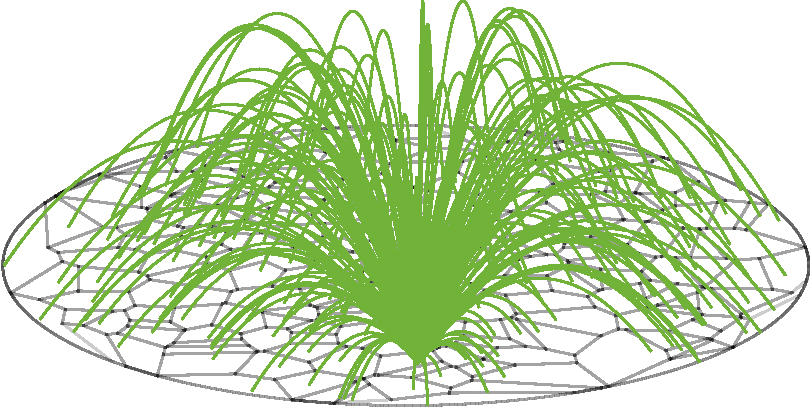
\includegraphics[width=0.4\textwidth]{gfx/chapter-monocentric/1.pdf}
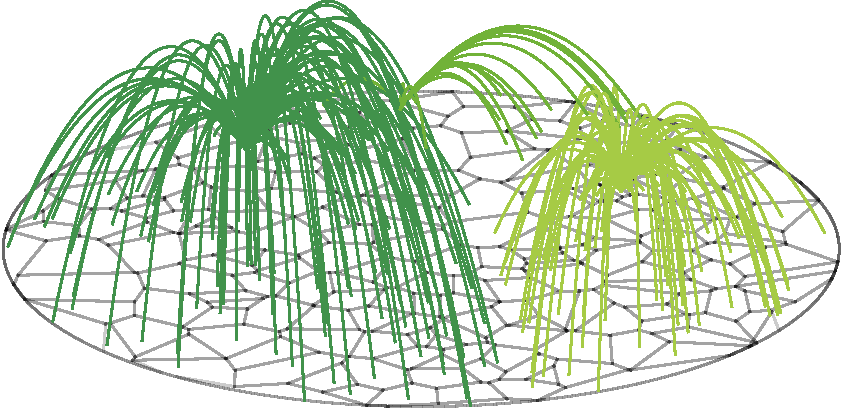
\includegraphics[width=0.4\textwidth]{gfx/chapter-monocentric/2.pdf}
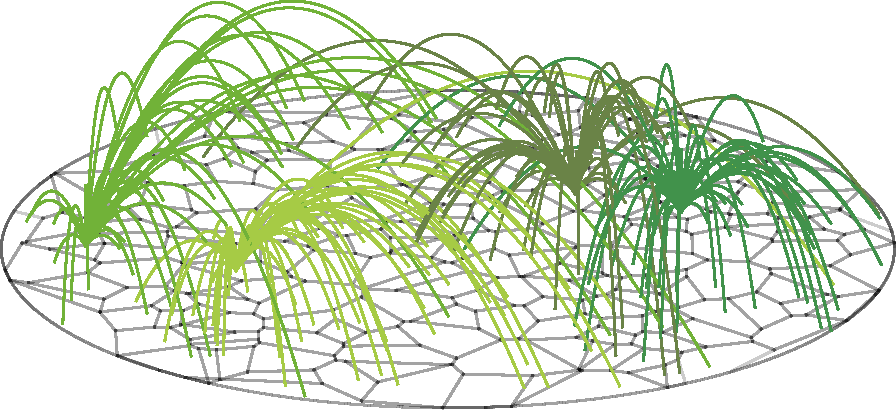
\includegraphics[width=0.4\textwidth]{gfx/chapter-monocentric/3.pdf}
\caption{The monocentric (top), distance-driven polycentric (middle)
  and attractivity-driven polycentric (bottom) regimes as produced by
  our model. Each link represents a commuting journey to an activity center. \label{fig:model_results}}
\end{figure}


From now on, we will assume that $\ell$ is large enough so that a
monocentric state exists for small values of the population. In this
regime, the value of $\eta$ prevails and the monocentric state evolves
to an attractivity-driven polycentric structure as the population
increases (if $\ell$ is too small, the monocentric regime does not
exist-see the Supplementary material~\cite{SM} for more details on
these points).  Starting from a small city with a monocentric
organisation, the traffic is negligible and $Z_{ij}\approx \eta_j$
which implies that all individual are going to choose the most
attractive center (with the largest value of $\eta_j$, say
$\eta_1$). When the number $P$ of households increases, the traffic
will also increase and some initially less attractive centers (with
smaller values of $\eta$) might become more attractive, leading to the
appearance of new subcenters characterized by a non-zero number of
commuters. More precisely, a new subcenter $j$ will appear when for an
individual $i$, we have $Z_{ij}>Z_{i1}$. The traffic so far is
$T(1)=P$ and $T(j)=0$ which leads to the equation
\begin{equation}
\eta_j-\frac{d_{ij}}{\ell}>\eta_1-\frac{d_{i1}}{\ell}\left[1+\left(\frac{P}{c}\right)^\mu\right]
\end{equation}
We assume that there are no spatial
correlations in the subcenter distribution, so that we can make the
approximation $d_{ij}\sim d_{i1}\sim L$. The new subcenter will thus
be such that $\eta_1-\eta_j$ is minimum implying that it will have the
second largest value denoted by $\eta_j=\eta_2$. For a uniform distribution
(details of the calculation can be found in the Supplementary
Material~\cite{SM}, section 2), on average
$\overline{\eta_1-\eta_2}\simeq 1/N_c$ leading to a critical value for
the population
%
\begin{equation}
P^*= c \left( \frac{\ell}{L N_c} \right)^{1/\mu}
\end{equation}
%
Whatever the system considered, there will therefore \emph{always} be
a critical value of the population above which the city becomes
polycentric (which can be smaller than one, in which case there is no
monocentric regime at all, see the Supplementary Material~\cite{SM}). The monocentric regime is therefore fundamentally
unstable with regards to population increase, which is in agreement with the fact that no major city in
the world exhibits a monocentric structure. We note that the smaller
the value of $\mu$ (or larger the value of the capacity $c$), the
larger the critical population value $P^*$ which means that cities
with a good road system capable of absorbing large traffic display a
monocentric structure for a longer period of time.


Having established that cities will eventually adopt a polycentric
structure, we can wonder how the number of subcenters varies with the
population. We compute the value of the population at which 
the $k^{th}$ center appears. We still assume that we are in the attractivity-driven regime and that, so far, $k-1$
centers have emerged with $\eta_{1} \geq \eta_{2} \geq ... \geq
\eta_{k-1}$~\cite{SM}, with a number of commuters $T(1), T(2), ...,
T(k-1)$, respectively. The next worker $i$ will choose the center $k$ if
\begin{equation}
Z_{ik} > \max_{j \in \left[1,k-1\right]} Z_{ij}
\end{equation}
which reads
\begin{equation}
\eta_k - \frac{d_{ik}}{\ell} > \max_{j \in \left[1,k-1\right]} \left\{
\eta_j - \frac{d_{ij}}{\ell} \left[ 1 + \left(
  \frac{T(j)}{c}\right)^\mu\right] \right\}
\end{equation}
The distribution of traffic $T(j)$ is narrow~\cite{SM}, which means that all the centers have roughly the same number of
commuters $T(j) \sim P/(k-1)$. As above we also assume that the
distance between the workers' households and the activity centers is
typically $d_{ij} \sim d_{ik} \sim L$. The previous expression now
reads
\begin{equation}
\frac{L}{\ell} \left( \frac{P}{(k-1)\,c} \right)^{\mu} > \max_{j \in
  \left[1,k-1\right]} \left( \eta_j \right) - \eta_k
\end{equation}
Following our definitions, $\max_{j \in \left[1,k-1\right]} \left(
\eta_j \right) = \eta_1$. According to order statistics, if the
$\eta_j$ are uniformly distributed, we have on average
$\overline{\eta_1 - \eta_k} = (k-1)/(N_c+1)$. It follows from these
assumptions that (1) the $k^{th}$ center to appear is the $k^{th}$ most attractive one (2) the average value of the population $\overline{P}_k$ at
which the $k^{th}$ center appears is given by:
%
\begin{equation}
\overline{P}_k = P^* \left( k-1 \right)^{\frac{\mu+1}{\mu}}
\label{eq:prediction}
\end{equation}
%
Conversely, the number $k$ of subcenters scales sublinearly with population as
\begin{equation}
k \sim \left( \frac{\overline{P}}{P^*} \right)^{\frac{\mu}{\mu + 1}}
\end{equation}
It is interesting to note that this result is robust: the dependence
is sublinear, \emph{whatever the distribution} of the random variable
$\eta$ (see the Supplementary Material~\cite{SM} for a discussion on this
point). We can therefore conclude that, probably very generally and
under mild assumptions, the number of activity subcenters in urban
areas scales sublinearly with their population where the prefactor and
the exponent depend on the properties of the transportation network of
the city under consideration. 

A previous study~\cite{Samaniego:2008} showed that the daily total
miles driven daily in a city --- the `total commuting
distance'---scales with the population as $L_{tot} \sim P^\gamma$
where $\gamma \in \left] 0.5, 1\right[$, which the authors interpreted
as cities having neither a neither totally centralized nor totally
decentralized structure. We can discuss this result within the
framework of our model in the following way. If the system was in the
pure attractivity-driven regime, we would have $L_{tot} \sim P$. But, if we
assume that we are in an intermediate regime where
Eq.~\ref{eq:prediction} holds, and where the system exhibits spatial
coherence~\cite{SM}, we can write the total length of commuting
journeys as
%
\begin{equation}
L_{tot} \sim P \frac{L}{\sqrt{k}}
\end{equation} 
%
Inverting the result from Eq.~\ref{eq:prediction} we therefore get
%
\begin{equation}
L_{tot} \sim P^{1-\frac{\beta}{2}}
\label{eq:beta}
\end{equation}
%
where $\beta = \frac{\mu}{\mu+1} \in \left[0 , 1\right]$. Our model is
thus consistent with the fact that the total traveled miles scales with
population with a non-trivial exponent comprised in $[0.5,1]$.\\


\begin{figure*}
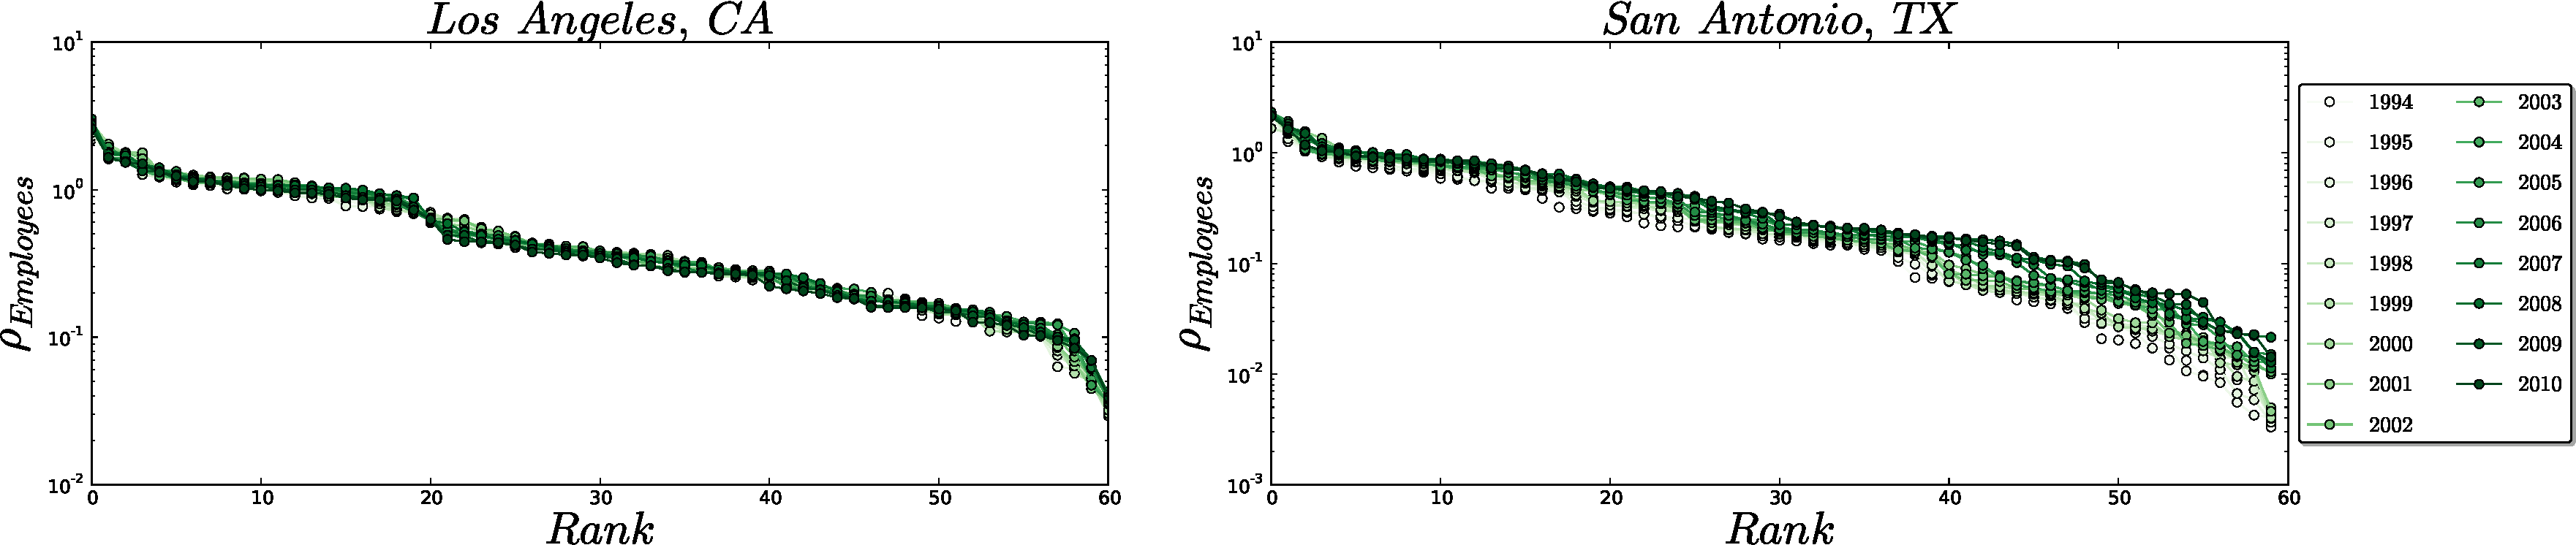
\includegraphics[width=\textwidth]{gfx/chapter-monocentric/4.pdf}
\caption{Rank-plot for the employment density (in employees per
  $km^2$) in Los Angeles, CA (left) and San Antonio, TX (right)
  between 1994 and 2010. See the Supplementary Material~\cite{SM} for more details. \label{fig:rank_plots}}
\end{figure*}

    \subsection{Empirical verification}
    \label{sub:empirical_verification}
    
People from the Census Bureau use the 2000 Census tract-to-tract commuting data
in order to get the employment density~\cite{Marlay:2010}. Use these data in
order to assess the employment density in 2000 MSAs. Use population data at the
same level in order to assess population density in 2000 MSAs.
Plot at several levels of the threshold and show the many different centers.
Propose a method to compute the number of centers (exponential, Loubar...).\\
        \subsubsection{Counting the number of centers}
        \label{ssub:counting_the_number_of_centers}
        
        
We now test the prediction given by Eq. (\ref{eq:prediction}). For
that purpose, we collected data for the number of employees per Zip
Codes in the United States for 16 years, between 1994 and
2010~\cite{ZBPdata}, as well as the population of all cities in the US
between 1994 and 2010~\cite{CensusData}. We estimate the number of
subcenters by constructing the rank-plot of the employment density
$\rho$ (number of employees per $km^2$) for each Zip Code of a given
urban area~\cite{Griffith:1981,Dokmeci:1994}. These plots display a decay as fast as an exponential
(Fig.~\ref{fig:rank_plots}) which implies that there exists a natural
scale for the rank, that we interpret here as the typical number of
activity centers. It also implies that any reasonable method should
give an estimate of the number of subcenters of the same order of
magnitude (which would not be the case for slowly decaying function
such as power laws for example). We first note that for some cities
--typically large ones with stable populations
(Fig.~\ref{fig:rank_plots}, left)-- the employment spatial statistics
remained stable over the period of study. For other cities, we observe
large variation of the number of subcenters
(Fig.~\ref{fig:rank_plots}, right). We then plot (Fig.~\ref{fig:data})
the population $P$ of cities (with population $P>100$) versus the
estimated number of subcenters $k$ (the dispersion in the scatterplot
probably results from the fact that different cities have different
resilience levels to congestion). On average, we observe a power law
dependance with exponent $\delta=1.56 \pm 0.15$ (the result is robust
with regards to the estimate of $k$, see the Supplementary
Material~\cite{SM} for more details). Inverting this relation gives us
the number of subcenters as a function of the population
%
\begin{equation}
k \sim P^{\beta}
\end{equation}
%
with $\beta \sim 0.64$. This result is strikingly in agreement with
the prediction given by our model: the number of subcenters in a city
scales sublinearly with its population.\\

\begin{figure}
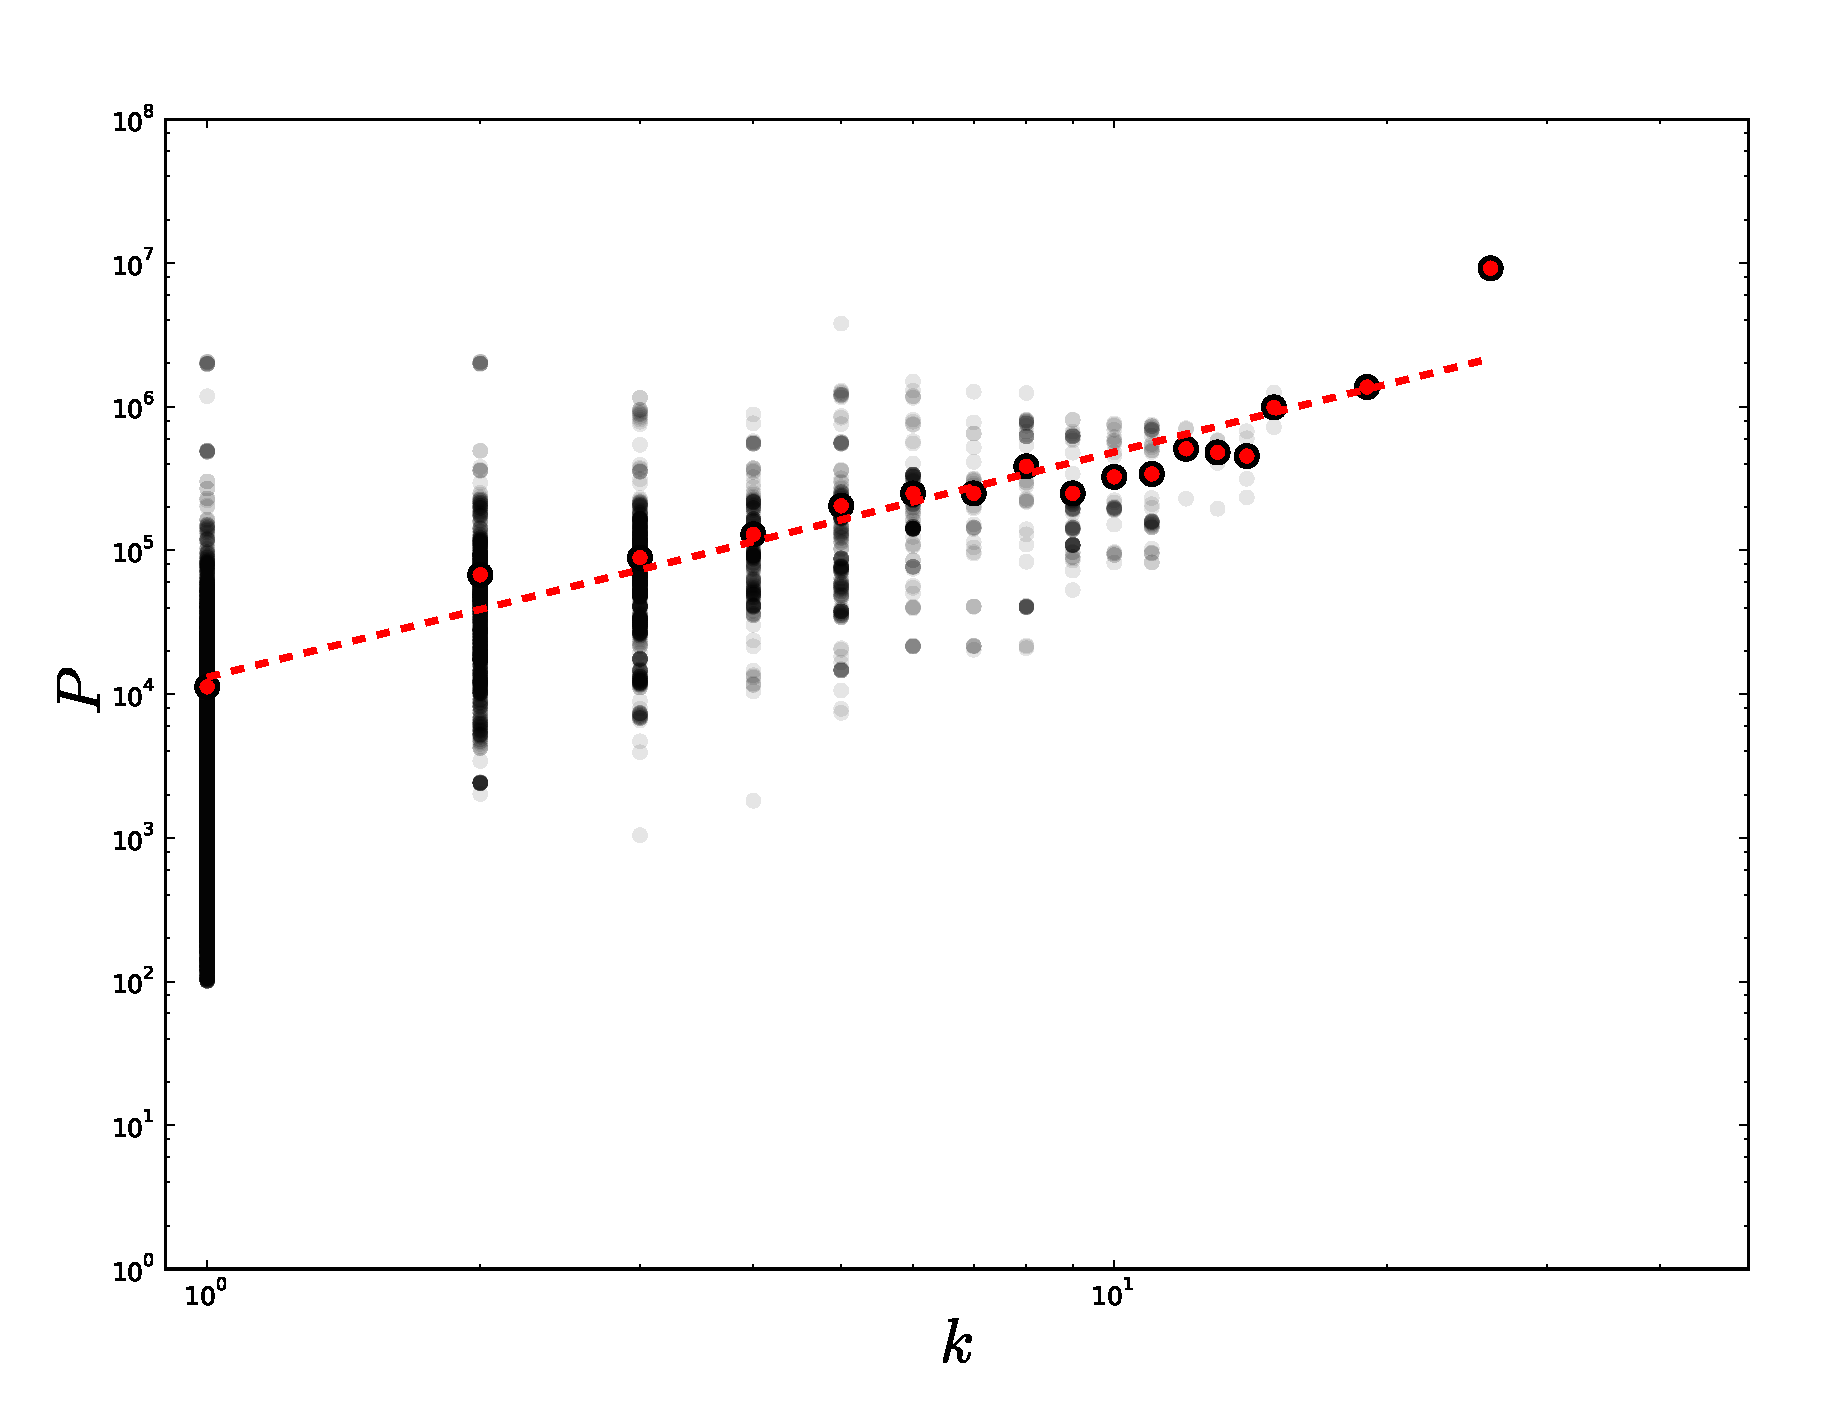
\includegraphics[width=0.5\textwidth]{gfx/chapter-monocentric/5.pdf}
\caption{Scatter plot of the estimated number of subcenters versus the
  population for about 9000 cities with population over 100 people in
  the US. The red dots represent the average population for a given
  number of subcenters. We fit this average with a power-law
  dependence (represented by a red dashed line) giving an exponent
  $\delta=1.56\pm 0.15$ ($r^2=0.87$). See the Supplementary Material~\cite{SM} for more details on the computation of $k$ and the robustness of the results. \label{fig:data}}
\end{figure}

Using the measured value of $\beta$ and Eq. (\ref{eq:beta}) we can estimate the exponent of
the scaling of $L_{tot}$ with the population and find $L_{tot} \sim
P^{\,0.68}$ which agrees very well with the value $0.66$ measured
in~\cite{Samaniego:2008} directly on the data of the daily total miles
driven in more than $400$ cities in the US.\\

While agglomeration economies seem to be the basic process explaining
the existence of cities and their spectacular resilience, this study
brings evidence that congestion is the driving force that tears them
apart. The non trivial spatial patterns observed in large cities can
thus be understood as a result of the interplay between these
competing processes. We believe that the present model represents an
important step towards a quantitative, predictive science of
cities. More generally, this microscopic approach is an interesting
example of an out-of-equilibrium model: it is governed by local
optimization with saturation effects, leads to different regimes, and
is characterized by non-trivial dynamical exponents. In this respect,
we believe that this discrete approach might be of use in the study of
pattern formation in biology --which have been so far explored from a
global optimisation perspective~\cite{Ashton:2005} or using
coarse-grained reaction-diffusion approaches with density dependent
diffusion coefficients~\cite{Cates:2012}-- to compute quantities that
are out of reach within the current methods.
\section{Proviso}
\label{sec:proviso}


 % Chapter 2

%------------------------------------------------

\ctparttext{Segregation is a notion that is difficult to define, hence the
extensive literature concerning segregation in the literature. In this part, we
propose to measure segregation as a deviation to the unsegregated city. We thus
provide a strong theoretical basis for the location coefficient. We further
derive a measure of attraction of the different categories, that allows us to
define unambiguously classes for the original categories. We study the
properties of neighbourhoods of different classes. We revisit the poor
center/rich suburb distinction. Finally, we propose a new measure of segregation
that takes space into account.} % Text on the Part 2 page describing the content in Part 2

\part{Socio-spatial stratification} % Second part of the thesis

% !TEX root = ../thesis-example.tex
%
\chapter{The socio-spatial stratification in cities}
\label{sec:concepts}


\begin{flushright}{\slshape    
The limits of my language\\
Are the limits of my world.} \\ \medskip
--- Ludwig Wittgenstein 
\end{flushright}

\section{Introduction}
\label{sec:introduction}

\section{Null model: the unsegregated city}
\label{sec:null_model_the_unsegregated_city}

\section{Measuring the attraction and repulsion of categories}
\label{sec:measuring_the_attraction_and_repulsion_of_categories}

\section{The emergent social classes}
\label{sec:the_emergent_social_classes}

\section{Clustering and concentration}
\label{sec:clustering_and_concentration}

\section{Poor centers, rich suburbs?}
\label{sec:poor_centers_rich_suburbs_}

\section{A new measure of segregation}
\label{sec:a_new_measure_of_segregation}
 % Chapter 2

%------------------------------------------------

\ctparttext{Cities and systems of cities are irrigated in people, energy,
information and goods thanks to various spatial networks. In this part, we show
how a new perspective on street patterns, and the use of OpenStreetMaps'
database allow us to provide a classification of cities based on their street
pattern. We then propose a large-scale description of subway and railway
networks, and are able to predict many of their properties based on the
properties of the underlying city or country.} % Text on the Part 2 page describing the content in Part 2

\part{Urban Networks} % Second part of the thesis

\include{chapters/chapter-networks} % Chapter 2


%------------------------------------------------

\ctparttext{Cities are not closed systems. Neither do they evolve in isolation.
Rather, they interact in what has been called a system of cities. In this part,
we focus on the movements of populations inside a system of city. We sutyd the
network of residential migrations in the US, describe some of its properties,
and show some unexpected consequences. Last, but not least, we show how Zipf's
law finds a natural explanation in when considering the motion of people.} % Text on the Part 2 page describing the content in Part 2

\part{Systems of cities} % Second part of the thesis

% !TEX root = ../thesis-example.tex
%
\chapter{The metropolitan blend}
\label{chap:metropolitan_blend}

\begin{flushright}{\slshape
You cannot base a general mathematical theory\\
on imprecisely defined concepts.\\
You can make some progress that way; \\
but sooner or later the theory is bound to dissolve in ambiguities\\ 
which prevent you from extending it further.} \medskip
--- E.T. Jaynesi~\cite{Jaynes:1986}
\end{flushright}
 % The metropolitan blend 
% !TEX root = ../thesis-example.tex
%
\chapter{Zipf's law and derivatives}
\label{chap:zipf_law}

 % Some work on Zipf
% !TEX root = ../thesis-example.tex
%
\chapter{The mystery of urban hierarchy}
\label{sec:concepts}

\begin{flushright}{\slshape    
The usual complaint about economic theory is that our models are
oversimplified---that offer excessively neat views of complex, messy reality.
[..] In one important case, the reverse is true: we have complex, messy models,
yet reality is startingly neat and simple.
} \\ \medskip
--- Paul Krugman~\cite{Krugman:1996}
\end{flushright}

\section{Introduction}
\label{sec:introduction}

\cite{Krugman:1996}
\cite{Gabaix:1999}
\cite{Batty:2013} for issues with Gibrat.
\cite{Cristelli:2012}
\cite{Batty:2006}

\section{The model}
\label{sec:the_model}


We write that 

\begin{equation}
    \partial_t P = \left(1-b-d\right)\,P + M_i^U + M_i^E
\end{equation} 

If the population is increasing wuch that

\begin{equation}
    P_{t+1} = \gamma_t\,P_t + \epsilon_t
\end{equation}

where $\epsilon_t$ is a small random increment with
$\mathrm{E}\left[\epsilon_t]\right] = \overline{\epsilon} > 0$. Whatever the
initial distirbution, the city-size distribution converges to a power-law with
and exponent $\zeta$ such that $\mathrm{E}\left[\gamma^\zeta\right] = 1$ (cite
Sornette). For small values of $\overline{\epsilon}$ we have

\begin{equation}
    \zeta = 1 + O(\epsilon)
\end{equation}

If the random variable is log-normally distributed, we have

\begin{equation}
    \zeta = 1 - \frac{2}{\sigma^2} \ln\left(1 -
    \frac{\overline{\epsilon}}{\overline{P}}\right)
\end{equation}

where $\overline{P}$ is the average size of a city. Therefore, the Zipf exponent
reads

\begin{equation}
    \boxed{    \alpha = \frac{1}{1 - \frac{2}{\sigma^2} \ln\left(1 -
\frac{\overline{\epsilon}}{\overline{P}}\right)}}
\end{equation}

From this equation one can clearly see that $\alpha > 1$ if and only if
$\overline{\epsilon} < 0$, that is when there is on average an outward flow
towards the outside of the system of cities (rural areas). On the other hand, we
have $\alpha < 1$ when $\overline{\epsilon} < 1$, that is when an important
rural exodus is happening, and $\alpha = 1$ if and only if $\overline{\epsilon}
= 0$, that is when the system of cities is at equilibrium with the rural
environment.
 % A model to explain Zipf's law

%------------------------------------------------

\ctparttext{In this part we summarize the results obtained in this thesis and
outline some possible future axes of research.} % Text on the Part 2 page describing the content in Part 2

\part{Conclusion} % Second part of the thesis

% !TEX root = ../thesis-example.tex
%
\chapter{Conclusion}
\label{sec:conclusion}

\begin{flushright}{\slshape    
If people never did silly things\\
nothing intelligent would ever get done.} \\ \medskip
--- Ludwig Wittgenstein 
\end{flushright}


\section{What the past 3 years have brought}
\label{sec:what_the_past_3_years_have_brought}


What I find striking is the propention of the different communities to ignore
one another. Although there is a lot to say about physicists being ignorant of
most of the literature in social sciences, there is also a lot to say about
social sciences applying tools as black boxes, without any reflexion on the
meaning of the formula that is being applied. Despite an important literature on
the topic, we can still see exponents of power-law distribution estimated using
the Least-Squares method. A lot of the litterature on complex network is also
applied carelessly, a big victim being the algorithms of community detection (no
reflection on the meaning of communities, for instance). It is a real shame,
because we need people with quantitative skills to manipulate formulas and
create new measures, but we also need qualitative skills to manipulate concept
and interpret the significance of the results. While we cannot expect a
physicist or a computer scientitist to know all the literature in a field that
is not his own, we cannot expect social scientists to have strong quantitative
skills. The real solution resides in the collaboration.\\

It is ignorance, not knowledge, that fuels science.

\section{The thesis I wish I wrote}
\label{sec:limitations}

The temptation is great, looking back on $3$ years of work with a more
experienced eye, to understate the contributions of this thesis and their
potential applications. The thesis that you have been reading is of course very
different from the thesis I would have liked to write. Frustrating realisation
that good research takes time. It takes time for the literature to sink in, it
takes time to understand the limits of your contribution, it takes time to get
at the bottom of a field. Not that I would do anything differently---I
couldn't--- but I now start to realise the work that is yet to be accomplished.
And that is only for what I am aware should be done, new problems and questions
are ready to pop out of nowhere at any time.\\

So what would have I write about---or at least try to---if I had to start my
thesis all over again? This is another way of saying: what are the next steps?
How does the research presented here fit in this picture?\\

I would start being more careful with the concepts that are being used. Starting
with the basics, with the single noun that was most often printed in these
pages: Cities. Despite it being our object study, it seems that the very
definition of this object is something obscure, somewhat hidden in the
literature. At least, it is something that is not really talked about in the
literature. Yet, if we want to exhibit robust empirical results, we need to
start worrying about the definition of the system we are studying. We need to
know \emph{what} cities we are talking about.\\


Once the boundaries are defined, we can start studying the way objects are
scattered within them. By objects, I mean buildings, roads, and first and
foremost people. The way we traditionally study the repartition of objects in
space is through the study of densities. An interesting thing to study would for
instance be the population density profile, possibly at different times of the
day. But density profiles are too complicated to comprehend for our brains,
especially when cities get large. Spatial statistics attemps to solve this
problem by providing simple measures, that extract a single number from
distributions. A single number is however too simple to be able to describe
accurately complex density profiles. What we need is a meso-scale
representation, somewhere between the micro-scale picture (the density profile
itself) and the macro-scale picture (a single number to summarize the density
profile). A requirement for this method is to make the definition of centers (or
hotspots) natural, because centers are a meso-scale representation of density
profiles already. This should make the notion of a center defined from first
principle, which would then allow to discuss the \emph{absolute} number of
centers in the city. Until now, because we do not clearly understand what the
meaning of the centers we obtain with the different existing methods, we are
only able to get numbers that are useful for inter-urban comparisons. The
spatial contiguity is not even taken into account!  This is where the model on
the polycentric transition of cities, presented in
Chapter~\ref{chap_monocentric} fits. Although I do not expect the scaling of the
number of centers with city size to change (but who knows), having a more
accurate description of the poly- or monocentric structure of population
distributions at different times of the day should help put more constrains on
existing models, and give hints for improvement of the existing models.\\


Once one is able to provide an accurate description of densit profiles, the
possibilities start to diverge. An obvious worry, when one has a picture of the
city's population at different times of the day, is the way these profile
transform one into another. This is linked to commuting---but not only,
commuting representing only $20\%$ of total travels in the
US~\cite{FHWA-PL-11-022}--- and the study of congestion of networks. We can
first wonder the link between the urban form (typically the residential and
employment densities) and mobility patterns. This is tackled in the excess
commuting literature (a few references here). There fit both the first and
second part of this thesis.\\ A futher worry linked to commuting is that of
congestion: understanding how congestion are formed, how they propagate and
devise strategies to mitigate them, either by influencing the transportation
infrastructure, the spatial repartition of residences and employment, or the
behaviour of people themselves.  This is far from being a recent worry, and
there already is an impressively vast literature on the topic [cite review].
Yet, there is room for new approaches that leverage the knowledge we have about
network and phase transition in physics. A first step in this direction has been
made by the authors of~\cite{Daqing:2015}, but there is surely more to be
understood and discovered.  Modeling congestion also implies understanding the
individual behaviour of people when they are moving from a point to another in
cities. Altough most research nowadays assume that people choose the shortest
(time or distance) path, GPS data now provide overwhelming evidence that this is
not the case [Manley, etc]. So, while there is a clear need to understand the
meso-scopic picture (how congestion spread), there is also is a critical need to
understand the microscopic picture (how people behave).\\

So far we have talked about the movement induced by the spatial mismatch between
residential areas and activity areas. One might also want to study the
characteristics of the spatial repartition of people. Inhabitants of cities are
not just a combination of a latitude and a longitude, a point on a map. Like you
and me, they are characterised by different qualities, some of which are
measurable: say their income, their education level, their ethnicity, etc. A
natural question, that has interested sociologist and geographers, is to wonder
whether people's residence is independent of these characteristics, or whether
these characteristics have an influence on the spatial repartition of
individuals. In other words, the study of residential segregation. A
contribution of this thesis is to provide a rigorous method to study the
patterns of segregation in the presence of multiple categories, and to identify
`neighbourhoods', that is regions in the city where individual belonging to a
particular category. I hope that, along with the improvement of the
characterisation of density profiles, we will be able to describe more
accurately the spatial patterns of segregation, which should hopefully lead to a
better understanding of this phenomenon, and better models.\\

The list is still long, and gets more and more speculative as we deviate from
the questions that are directly entailed by the work I have presented here.


\section{Future work}
\label{sec:future_work}

I do believe there is a cruel lack of serious empirical work in the field. This
should be quickly solved, thanks to the information technologies that are now
available. But there is a bigger problem looming over our heads. The
uncomfortable fact that our fundamental object, the city, is an ill-defined
object. And that most empirical studies possibly rely on definitions of a city
that are not suited to the study they undertake. 
This lack of serious definition compromises the comparison between cities of
different countries (as I saw in the fingerprint paper), or different points in
time. I am, of course, not the first person to acknowledge this empirical
difficulty. In fact, it has been a long-time worry of geographers who have been
trying to produce harmonised database for a long time (cite
Bretagnolle, Pumain, any reference on harmonised database). Yet, we still lack
of an unambiguous, theoretically grounded definition of what a city is. And this
is problematic, since statistical institutes' results are based on what is
believed to be the best definition of the city at a time, which influences the
results, etc.
The problem is that it is unlikely there is only one way to define the object
city, but rather different definitions that depend on what we are studying.
People are usually confused by the existence of different definitions.


 % Chapter 2


%----------------------------------------------------------------------------------------
%	THESIS CONTENT - APPENDICES
%----------------------------------------------------------------------------------------

%\appendix

%\part{Appendix} % New part of the thesis for the appendix

%\include{Chapters/Chapter0A} % Appendix A
%\include{Chapters/Chapter0B} % Appendix B - empty template

%----------------------------------------------------------------------------------------
%	POST-CONTENT THESIS PAGES
%----------------------------------------------------------------------------------------

\cleardoublepage% Bibliography

\label{app:bibliography} % Reference the bibliography elsewhere with \autoref{app:bibliography}

\manualmark
\markboth{\spacedlowsmallcaps{\bibname}}{\spacedlowsmallcaps{\bibname}} 
\refstepcounter{dummy}

\addtocontents{toc}{\protect\vspace{\beforebibskip}} % Place the bibliography slightly below the rest of the document content in the table of contents
\addcontentsline{toc}{chapter}{\tocEntry{\bibname}}

\bibliographystyle{plainnat}

\bibliography{Bibliography} % Bibliography

\cleardoublepage% Colophon (a brief description of publication or production notes relevant to the edition)

\pagestyle{empty}

\hfill

\vfill

\pdfbookmark[0]{Colophon}{colophon}

\section*{Colophon}

This document was typeset using the typographical look-and-feel \texttt{classicthesis} developed by Andr\'e Miede. The style was inspired by Robert Bringhurst's seminal book on typography ``\emph{The Elements of Typographic Style}''. \texttt{classicthesis} is available for both \LaTeX\ and \mLyX: 

\begin{center}
\url{http://code.google.com/p/classicthesis/}
\end{center}

\noindent Happy users of \texttt{classicthesis} usually send a real postcard to the author, a collection of postcards received so far is featured here: 

\begin{center}
\url{http://postcards.miede.de/}
\end{center}
 
\bigskip

\noindent\finalVersionString % Colophon

\cleardoublepage% Declaration

\refstepcounter{dummy}
\pdfbookmark[0]{Declaration}{declaration} % Bookmark name visible in a PDF viewer

\chapter*{Declaration} % Declaration section text

\thispagestyle{empty}

Put your declaration here.
\bigskip
 
\noindent\textit{\myLocation, \myTime}

\smallskip

\begin{flushright}
\begin{tabular}{m{5cm}}
\\ \hline
\centering\myName, \today \\
\end{tabular}
\end{flushright}
 % Declaration

%----------------------------------------------------------------------------------------

\end{document}
